\section{EXTRAPOLATIONS TO THE PHYSICAL LIMIT}
\label{sec:physical_limit_extrapolation}

\subsection{Motivation for the \texorpdfstring{$\hat{\zeta} \to \infty$}{TEXT} Extrapolation}
\label{sec:zetahat_extrapolation_motivation}

Section~\ref{sec:fitting_methodologies} established stable global simultaneous fits to the invariant amplitudes $\tAmp_{2B}$ and $\tAmp_{12B}$ at each of our four simulated nucleon momenta, corresponding to the finite Collins-Soper parameters $\hat\zeta = 0.090772,\ 0.294367,\ 0.539684,\ 0.785756$ for $P_L=-1,-2,-3,-4$ respectively (Table~\ref{tab:zeta_directions}). As discussed in Section~\ref{sec:collins_soper_parameter}, these finite-$\hat\zeta$ results are a consequence of the space-like staple direction required by our Euclidean lattice geometry; the physical, light-cone TMDs are recovered only in the limit $\hat\zeta \to \infty$. Before our lattice results can be compared to phenomenological extractions of the Sivers function, each finite-momentum result must therefore be extrapolated to this physical limit.

Figure~\ref{fig:zetahat_discrete_slices} shows why this extrapolation is necessary in practice. At fixed transverse quark separation $|b_T| = 3a \approx 0.34$ fm, we evaluate the reconstructed amplitudes $\tAmp_{2B}^{\text{Re}}$ and $i\tAmp_{2B}^{\text{Im}}$, the corresponding unpolarized and Sivers TMD combinations $\tilde f_1^{(0)} = 2\tAmp_{2B}$ and $\tilde f_1^{\perp(1)} = -2\tAmp_{12B}$, and the resulting Sivers shift $\langle k_y \rangle_{TU}$ and $x\langle k_y \rangle_{TU}$, as continuous functions of $x$ at each of our four simulated momenta. Plotting these six quantities against $1/\hat\zeta$ shows that every one of them varies systematically with the momentum: none of our finite lattice momenta has yet reached the physical limit, and the extrapolation to $1/\hat\zeta \to 0$ carried out in the remainder of this chapter is required before the results can be interpreted physically.

\begin{figure}[h!]
    \centering
    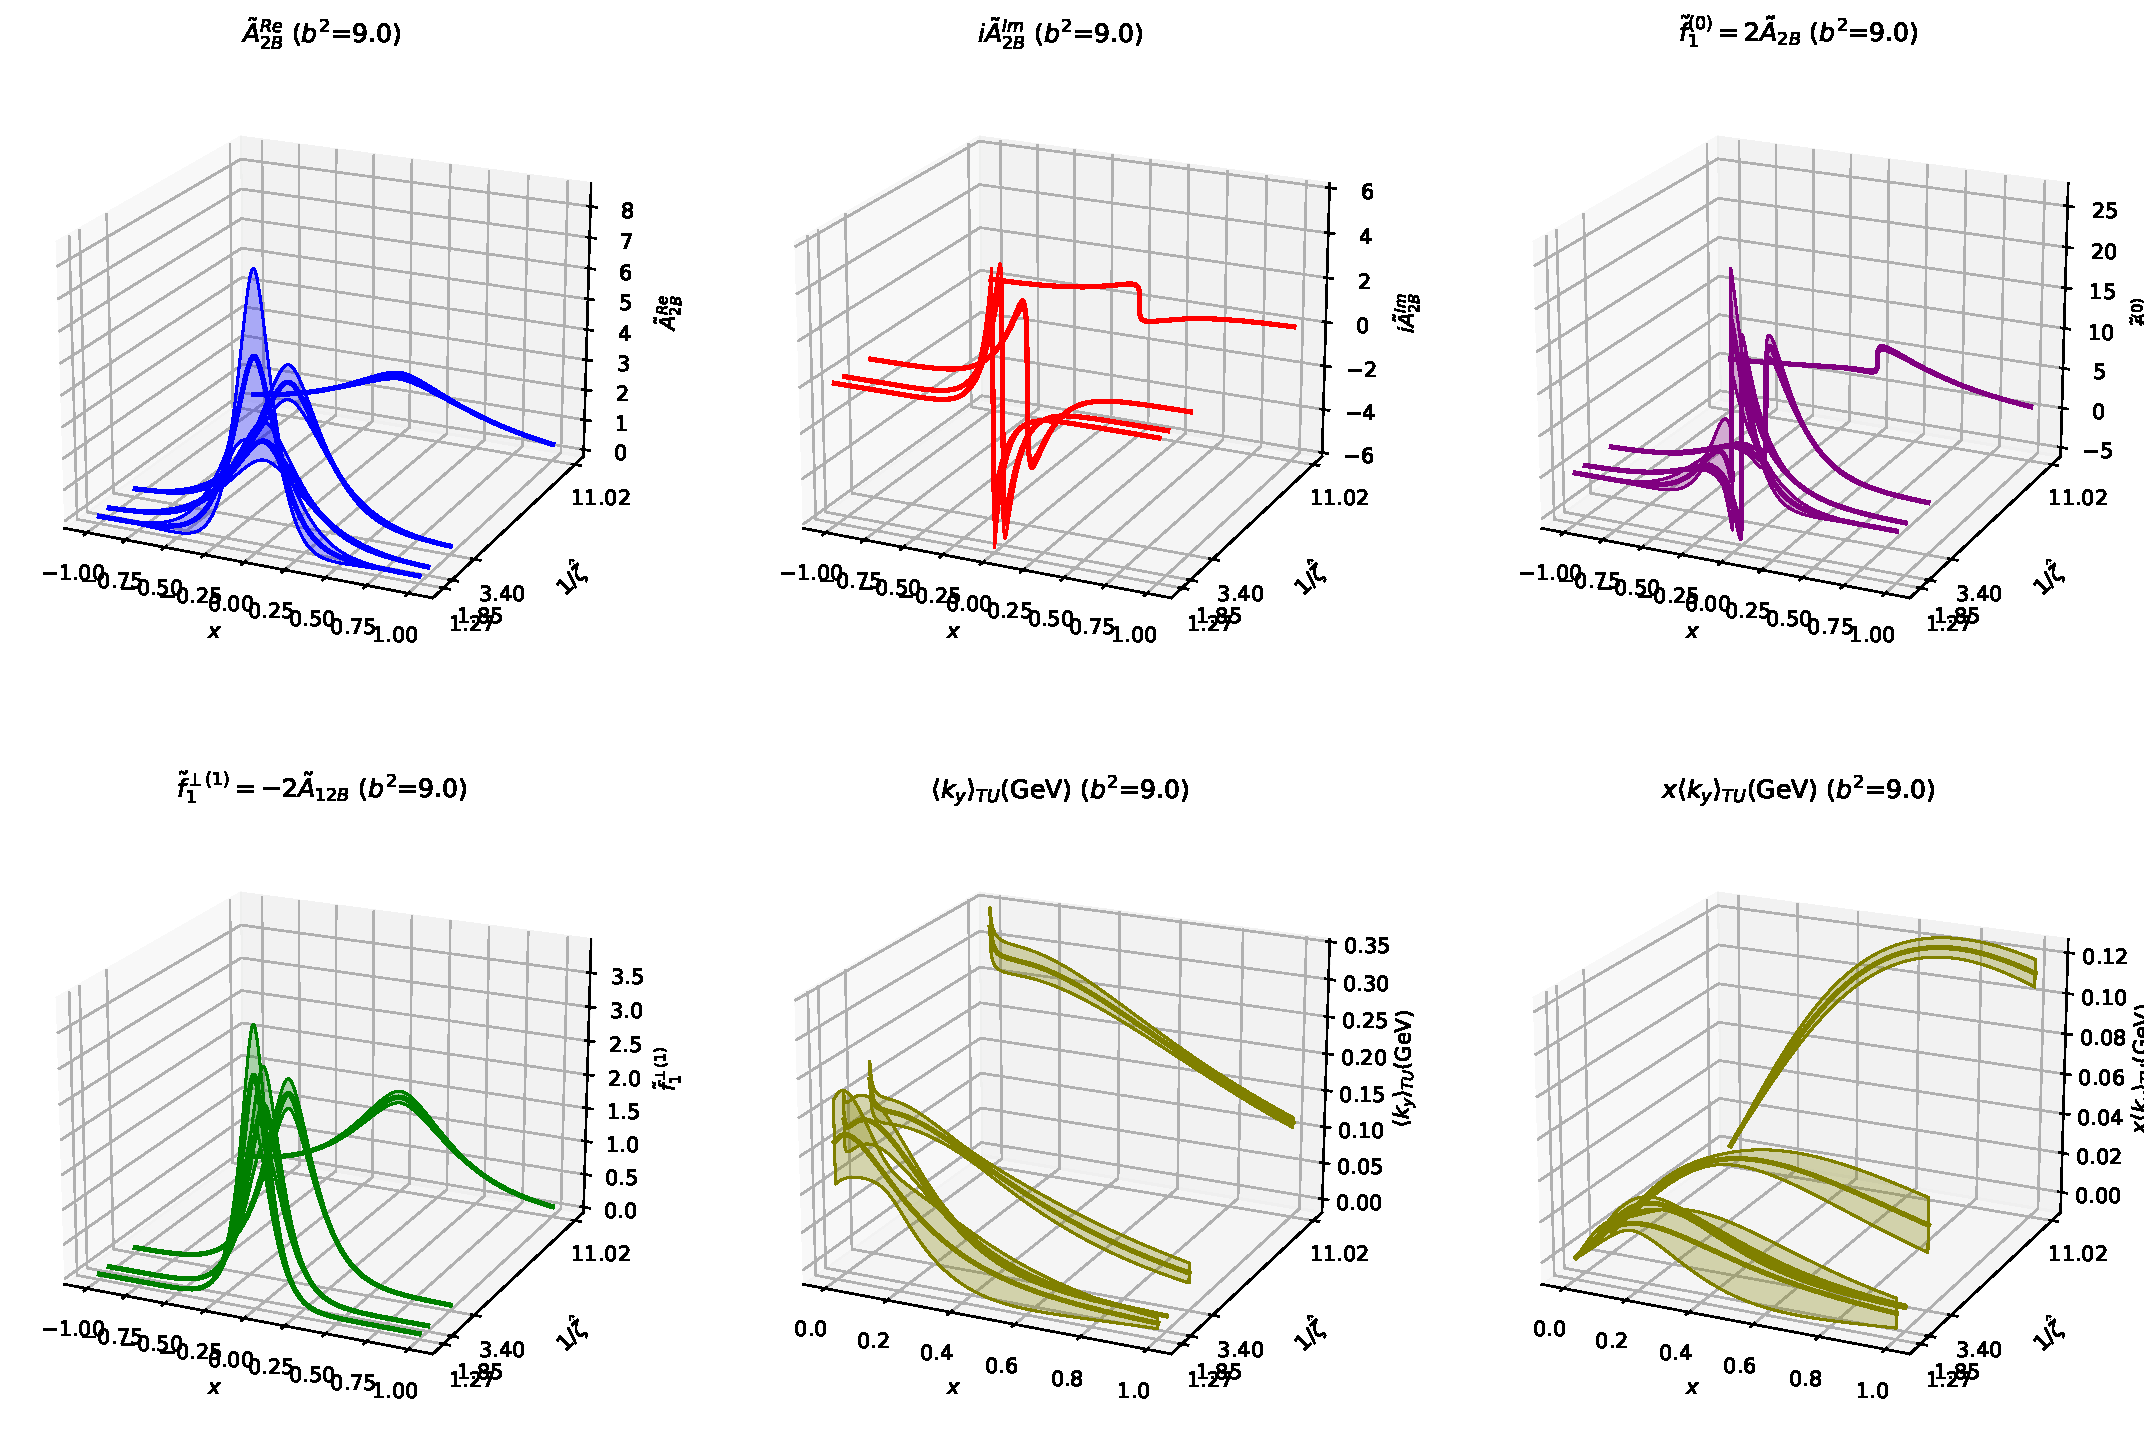
\includegraphics[width=0.8\linewidth]{SimultaneousFitsCov/SimulFit_Distinct_1_over_PL_bmin3_eta610_b29.0.pdf}
    \caption{Discrete $\hat\zeta$-slices of the reconstructed amplitudes, unpolarized and Sivers TMD combinations, and Sivers shift, plotted against both $x$ and $1/\hat\zeta$ at fixed transverse separation $|b_T| = 3a \approx 0.34$ fm. Each ribbon corresponds to one of the four simulated momenta $P_L = -1,-2,-3,-4$ (equivalently $1/\hat\zeta = 11.02,\ 3.40,\ 1.85,\ 1.27$). The systematic drift of every panel with $1/\hat\zeta$ motivates the extrapolation to the physical light-cone limit $\hat\zeta \to \infty$ performed below.}
    \label{fig:zetahat_discrete_slices}
\end{figure}

\subsection{Extrapolation at fit-parameters level}
\label{sec:extrap_fit_param_level}

The lowest simulated momentum, $P_L=-1$ ($\hat\zeta = 0.090772$), sits too close to the origin in $1/\hat\zeta$ to resolve the curvature required to anchor an extrapolation; including it risks biasing the fit away from the true asymptotic ($\hat\zeta \to \infty$) behavior rather than constraining it. We therefore exclude $P_L=-1$ and extrapolate using only the three higher, better-separated momenta $P_L = -2,-3,-4$.

Rather than extrapolate the amplitudes point by point in $x$, we extrapolate each of the twelve parameters of the global simultaneous-fit models directly: the four parameters $\{a,c,d,j\}$ appearing in each of the coupled Lorentzian models for $\tAmp_{2B}^{\text{Re}}$, $\tAmp_{2B}^{\text{Im}}$, and $\tAmp_{12B}^{\text{Re}}$ (Eq.~(\ref{eq:model_ReA2B})-(\ref{eq:model_ImA2B})). Following the kinematic scaling identified in Section~\ref{sec:fitting_methodologies}, the parameters $c_{\text{re}}$, $c_{\text{im}}$, and $c_{\text{reA12B}}$ are first rescaled by $1/P_L^2$ and $a_{\text{im}}$ by $1/P_L$, so that all three momenta can be fit on a common footing. For the resulting $\hat\zeta$-dependence of each rescaled parameter, we tested two functional forms,
\begin{equation}
    p(\hat\zeta) = c + \frac{d}{\hat\zeta} \qquad \text{and} \qquad p(\hat\zeta) = c + \frac{d}{\hat\zeta^2} \ ,
    \label{eq:zetahat_extrap_ansatz}
\end{equation}
using correlated Jackknife fits to the three data points. The quadratic ansatz consistently gave a lower $\chi^2/\text{dof}$ across the twelve parameters than the linear form and is adopted for every extrapolation shown below; the extrapolated, physical-limit value of each parameter is simply its fitted intercept $c$ at $1/\hat\zeta=0$.

\begin{figure}[h!]
    \centering
    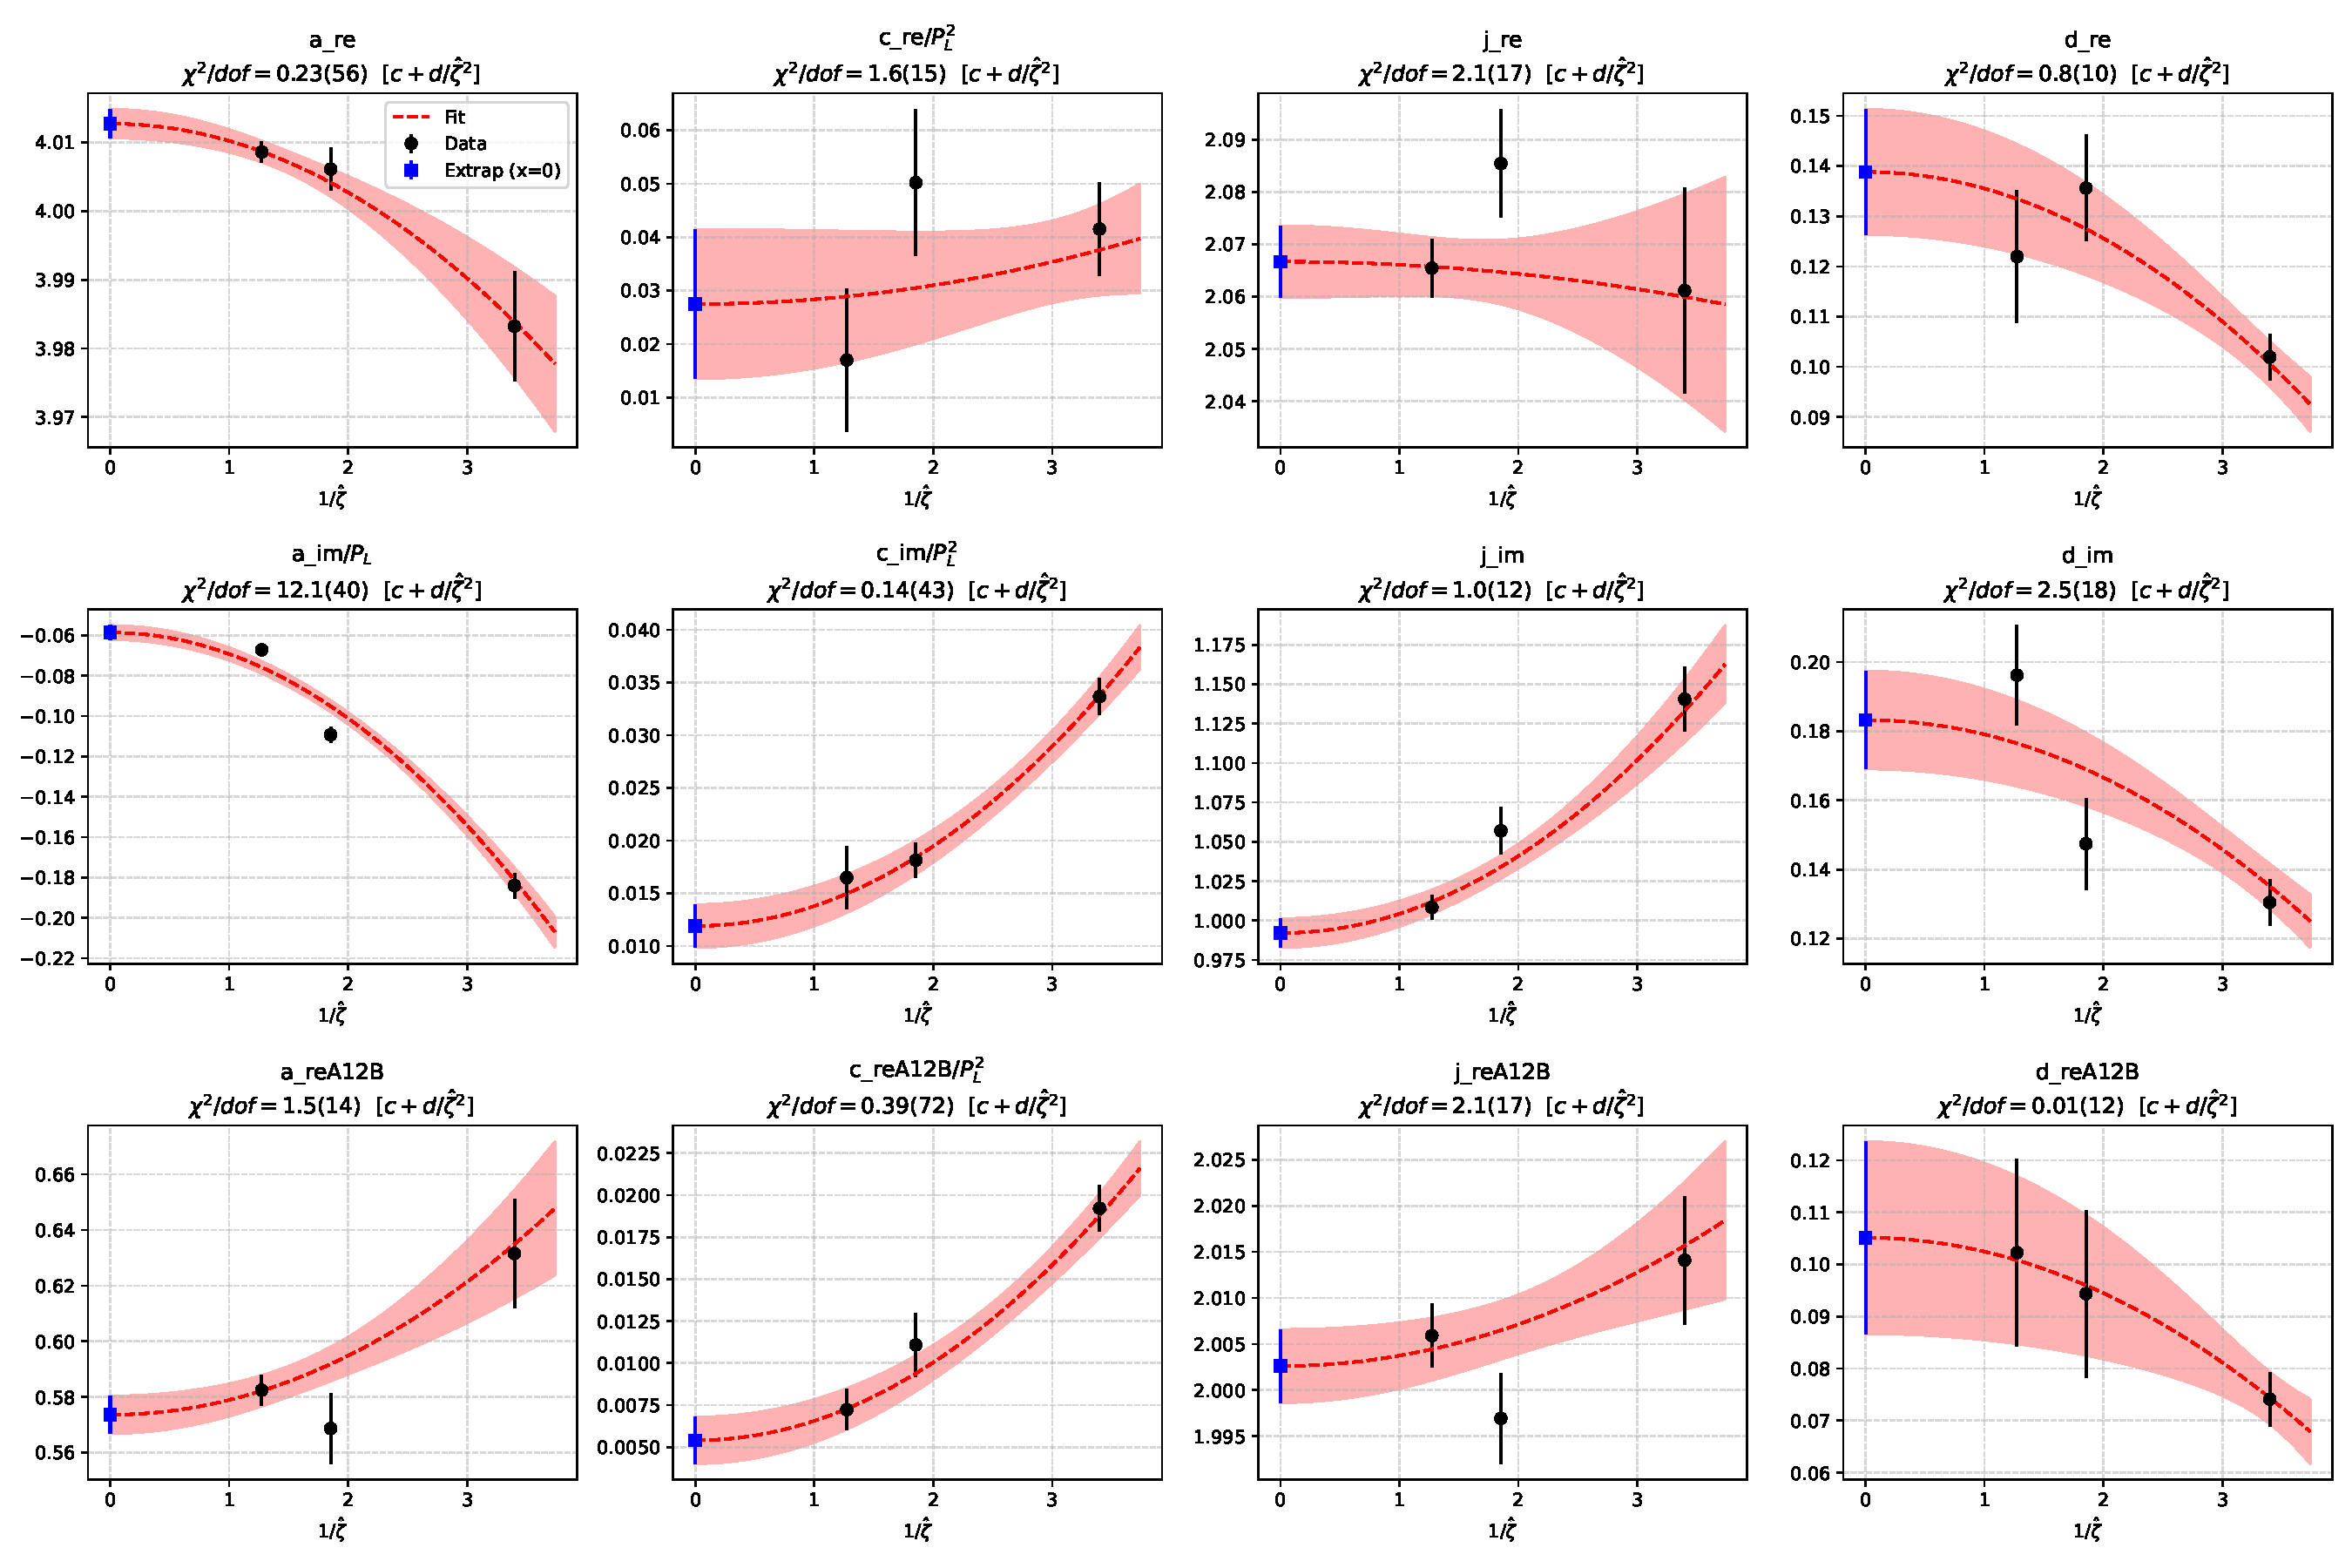
\includegraphics[width=0.8\linewidth]{SimultaneousFitsCov/extrapolation_para_level/Param_Extrapolations_1byZetahat_sq_P234_bmin3_eta610_b29.0.pdf}
    \caption{Extrapolation of the twelve simultaneous-fit parameters to the physical limit $\hat\zeta \to \infty$, using only the three higher momenta $P_L=-2,-3,-4$ (black points, plotted against $1/\hat\zeta$). The dashed red curve and shaded band show the fitted ansatz $c+d/\hat\zeta^2$ of Eq.~\ref{eq:zetahat_extrap_ansatz}, with each panel's Jackknife $\chi^2/\text{dof}$ noted in its title; the blue square at $1/\hat\zeta=0$ marks the extrapolated physical-limit value. The parameters $c_{\text{re}}$, $c_{\text{im}}$, and $c_{\text{reA12B}}$ are shown rescaled by $1/P_L^2$, and $a_{\text{im}}$ by $1/P_L$, as described in the text.}
    \label{fig:param_extrapolation_zetahat}
\end{figure}

Reconstructing the amplitudes from these twelve extrapolated parameters gives the unpolarized and Sivers TMD combinations directly at the physical limit, shown in Fig.~\ref{fig:extrapolated_amplitude_level} as continuous functions of $x$ at fixed $|b_T| = 3a \approx 0.34$ fm.

\begin{figure}[h!]
    \centering
    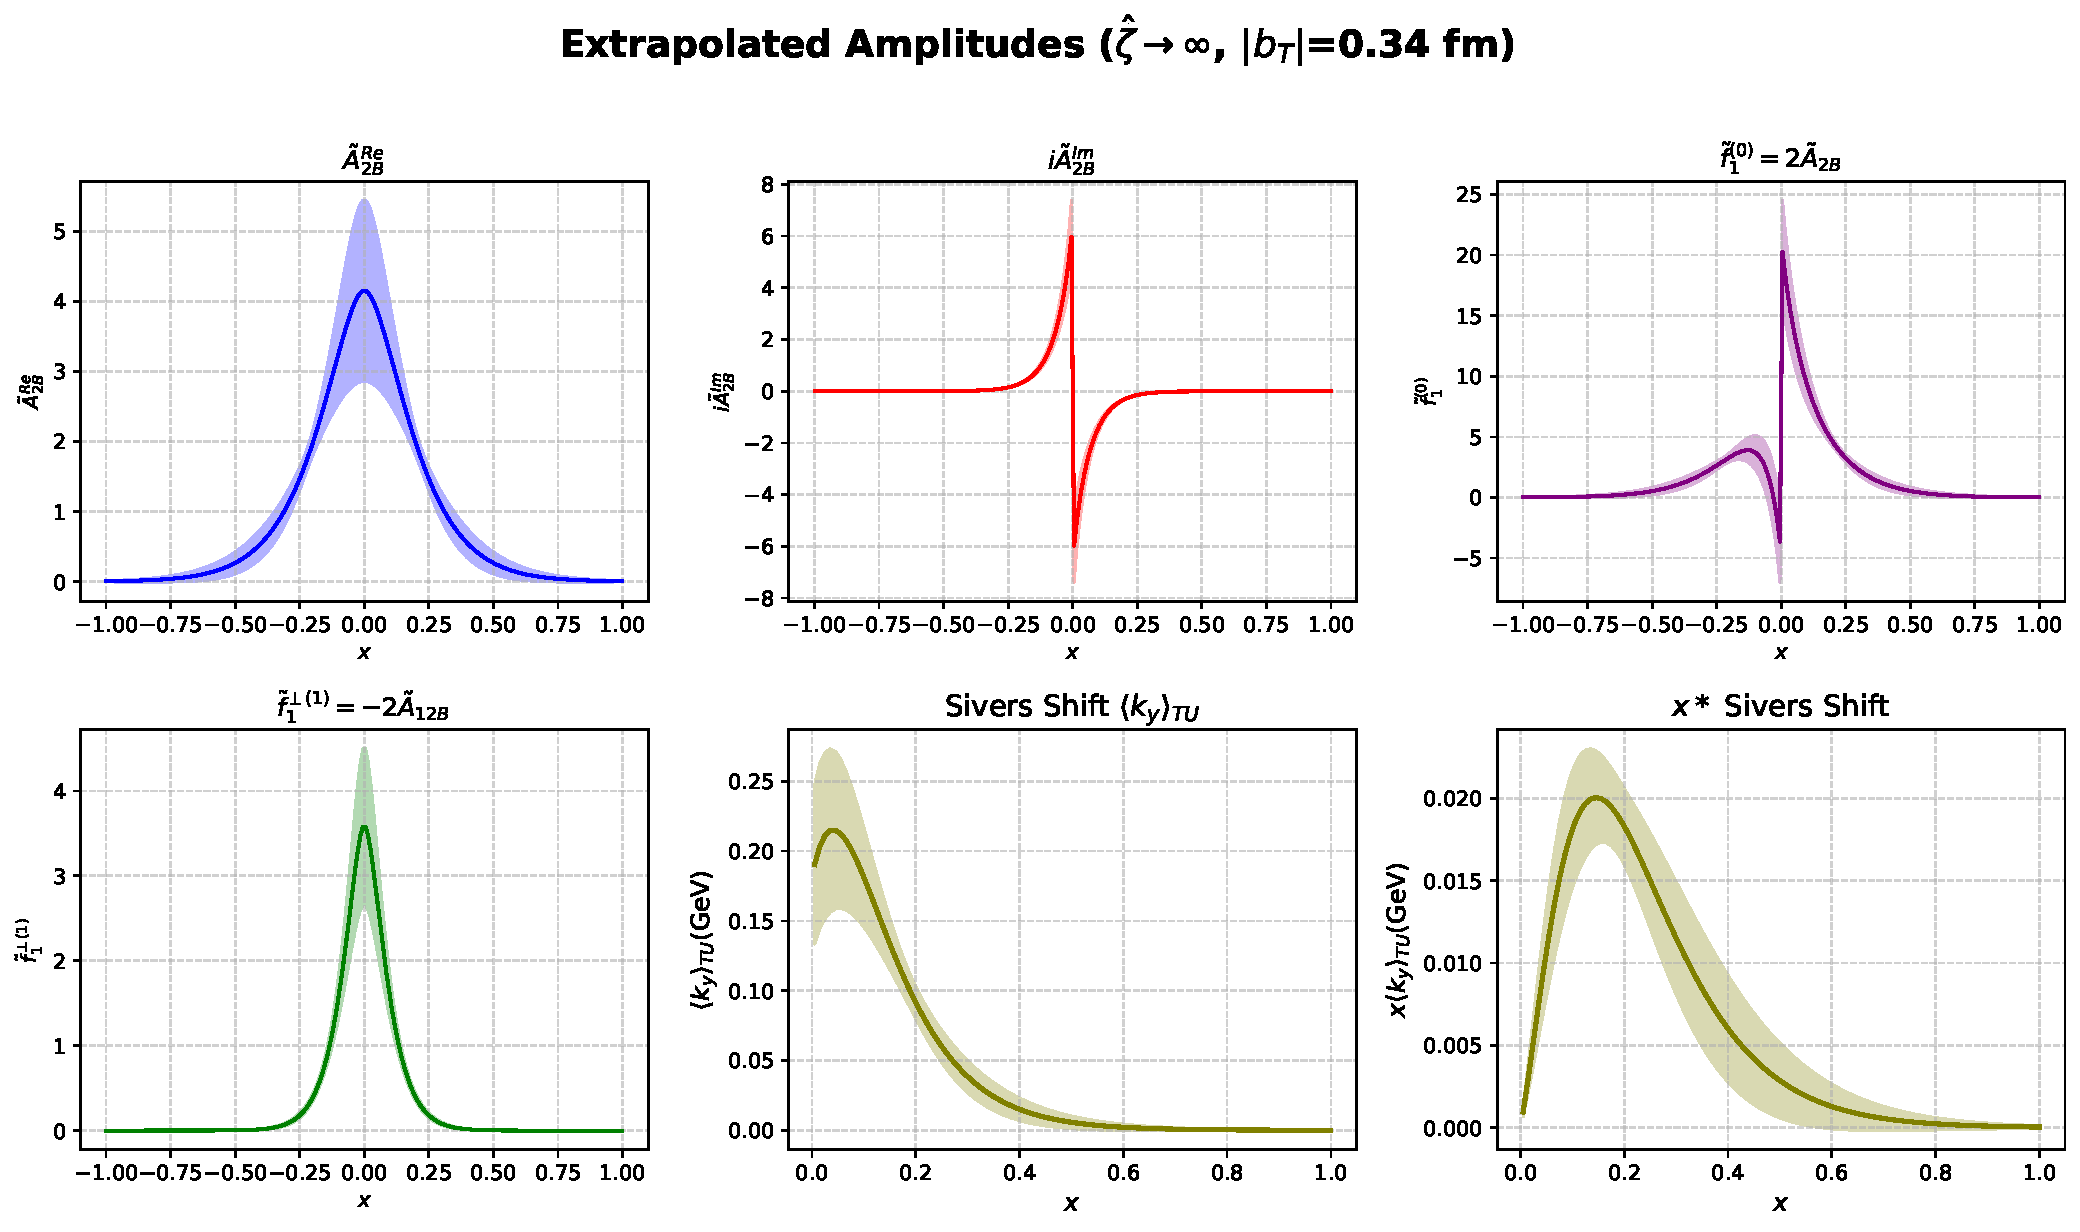
\includegraphics[width=0.8\linewidth]{SimultaneousFitsCov/extrapolation_para_level/Extrapolated_AmpLevel_P234_Sivers_1_over_zetahat_sq_bmin3_eta610_b29.0.pdf}
    \caption{Unpolarized and Sivers TMD amplitudes reconstructed from the extrapolated ($\hat\zeta\to\infty$) fit parameters of Fig.~\ref{fig:param_extrapolation_zetahat}, evaluated as continuous functions of $x$ at fixed transverse separation $|b_T| = 3a \approx 0.34$ fm: $\tAmp_{2B}^{\text{Re}}$, $i\tAmp_{2B}^{\text{Im}}$, the full unpolarized combination $\tilde f_1^{(0)}=2\tAmp_{2B}$, the Sivers combination $\tilde f_1^{\perp(1)}=-2\tAmp_{12B}^{\text{Re}}$, and the resulting Sivers shift $\langle k_y \rangle_{TU}$ and $x\langle k_y \rangle_{TU}$, the latter two restricted to the quark region $x\ge0$. Shaded bands are the Jackknife uncertainty propagated from the twelve extrapolated parameters.}
    \label{fig:extrapolated_amplitude_level}
\end{figure}

Table~\ref{tab:numerical_integration_fourier} lists the corresponding numerical Fourier-transform integrals at $|b_T|=3a\approx0.34$ fm, evaluated over the full range $x\in\{-\infty,\infty\}$ as well as the restricted ranges $\{-1,1\}$, $\{-1,0\}$, and $\{0,1\}$ used to isolate, respectively, the quark-plus-antiquark, antiquark, and quark contributions to the $x$-moments $\tilde f_1^{[1](0)}$ and $\tilde f_{1T}^{\perp[1](1)}$.

\begin{table}[h!]
    \centering
    \renewcommand{\arraystretch}{1.5}
    \caption{Numerical integration of the Fourier-transform integrals at $|b_T| = 3a \approx 0.34$ fm, evaluated using the extrapolated ($\hat\zeta\to\infty$) amplitudes of Fig.~\ref{fig:extrapolated_amplitude_level}, over the full range and three restricted $x$-ranges isolating the quark, antiquark, and combined contributions.}
    \label{tab:numerical_integration_fourier}
    \resizebox{\textwidth}{!}{%
    \begin{tabular}{|l|c|c|c|c|}
    \hline
    Integral & $\{-\infty,\infty\}$ & $\{-1,1\}$ & $\{-1,0\}$ & $\{0,1\}$ \\
    \hline
    $\displaystyle\int dx\, \tAmp_{2B}^{\text{Re}}$ & $1.88(20)$ & $1.88(20)$ & $0.941(100)$ & $0.941(100)$ \\
    \hline
    $\displaystyle\int dx\, (i\tAmp_{2B}^{\text{Im}})$ & $2(23)\times10^{-16}$ & $7(52)\times10^{-16}$ & $0.413(68)$ & $-0.423(72)$ \\
    \hline
    $\tilde f_1^{[1](0)} = 2\displaystyle\int dx\, (\tAmp_{2B}^{\text{Re}} - i\tAmp_{2B}^{\text{Im}})$ & $3.77(40)$ & $3.76(40)$ & $1.06(20)$ & $2.73(28)$ \\
    \hline
    $\tilde f_{1T}^{\perp[1](1)} = -2\displaystyle\int dx\, \tAmp_{12B}^{\text{Re}}$ & $0.76(13)$ & $0.76(13)$ & $0.379(67)$ & $0.379(67)$ \\
    \hline
    $\mN\,\dfrac{\tilde f_{1T}^{\perp[1](1)}}{\tilde f_1^{[1](0)}}$ & $0.217(38)$ & $0.217(38)$ & $0.387(89)$ & $0.150(26)$ \\
    \hline
    \end{tabular}%
    }
\end{table}

Restricting the integration to $x\in\{-1,0\}$ or $\{0,1\}$ isolates the antiquark and quark contributions respectively; because $\tAmp_{2B}^{\text{Im}}$ is an odd function of $x$ while $\tAmp_{2B}^{\text{Re}}$ and $\tAmp_{12B}^{\text{Re}}$ are even, the antiquark and quark ranges give equal $\int dx\,\tAmp_{2B}^{\text{Re}}$ and $\int dx\,\tAmp_{12B}^{\text{Re}}$ but opposite-sign $\int dx\,(i\tAmp_{2B}^{\text{Im}})$, so that the combined $\{-1,1\}$ integral of the imaginary term is consistent with zero to within uncertainty. Integrating over the full range $\{-\infty,\infty\}$ agrees with the physically motivated range $\{-1,1\}$ well within uncertainties, confirming that the extrapolated amplitudes decay fast enough in $x$ for the light-cone-momentum-fraction cutoff to be a negligible truncation.

Figure~\ref{fig:extrapolated_amplitude_3d} extends this reconstruction to the full dependence on both $x$ and transverse separation, while Fig.~\ref{fig:momenta_vs_extrapolated} compares the extrapolated result directly against each of the three finite momenta used to obtain it.

\pagebreak
\begin{figure}[h!]
    \centering
    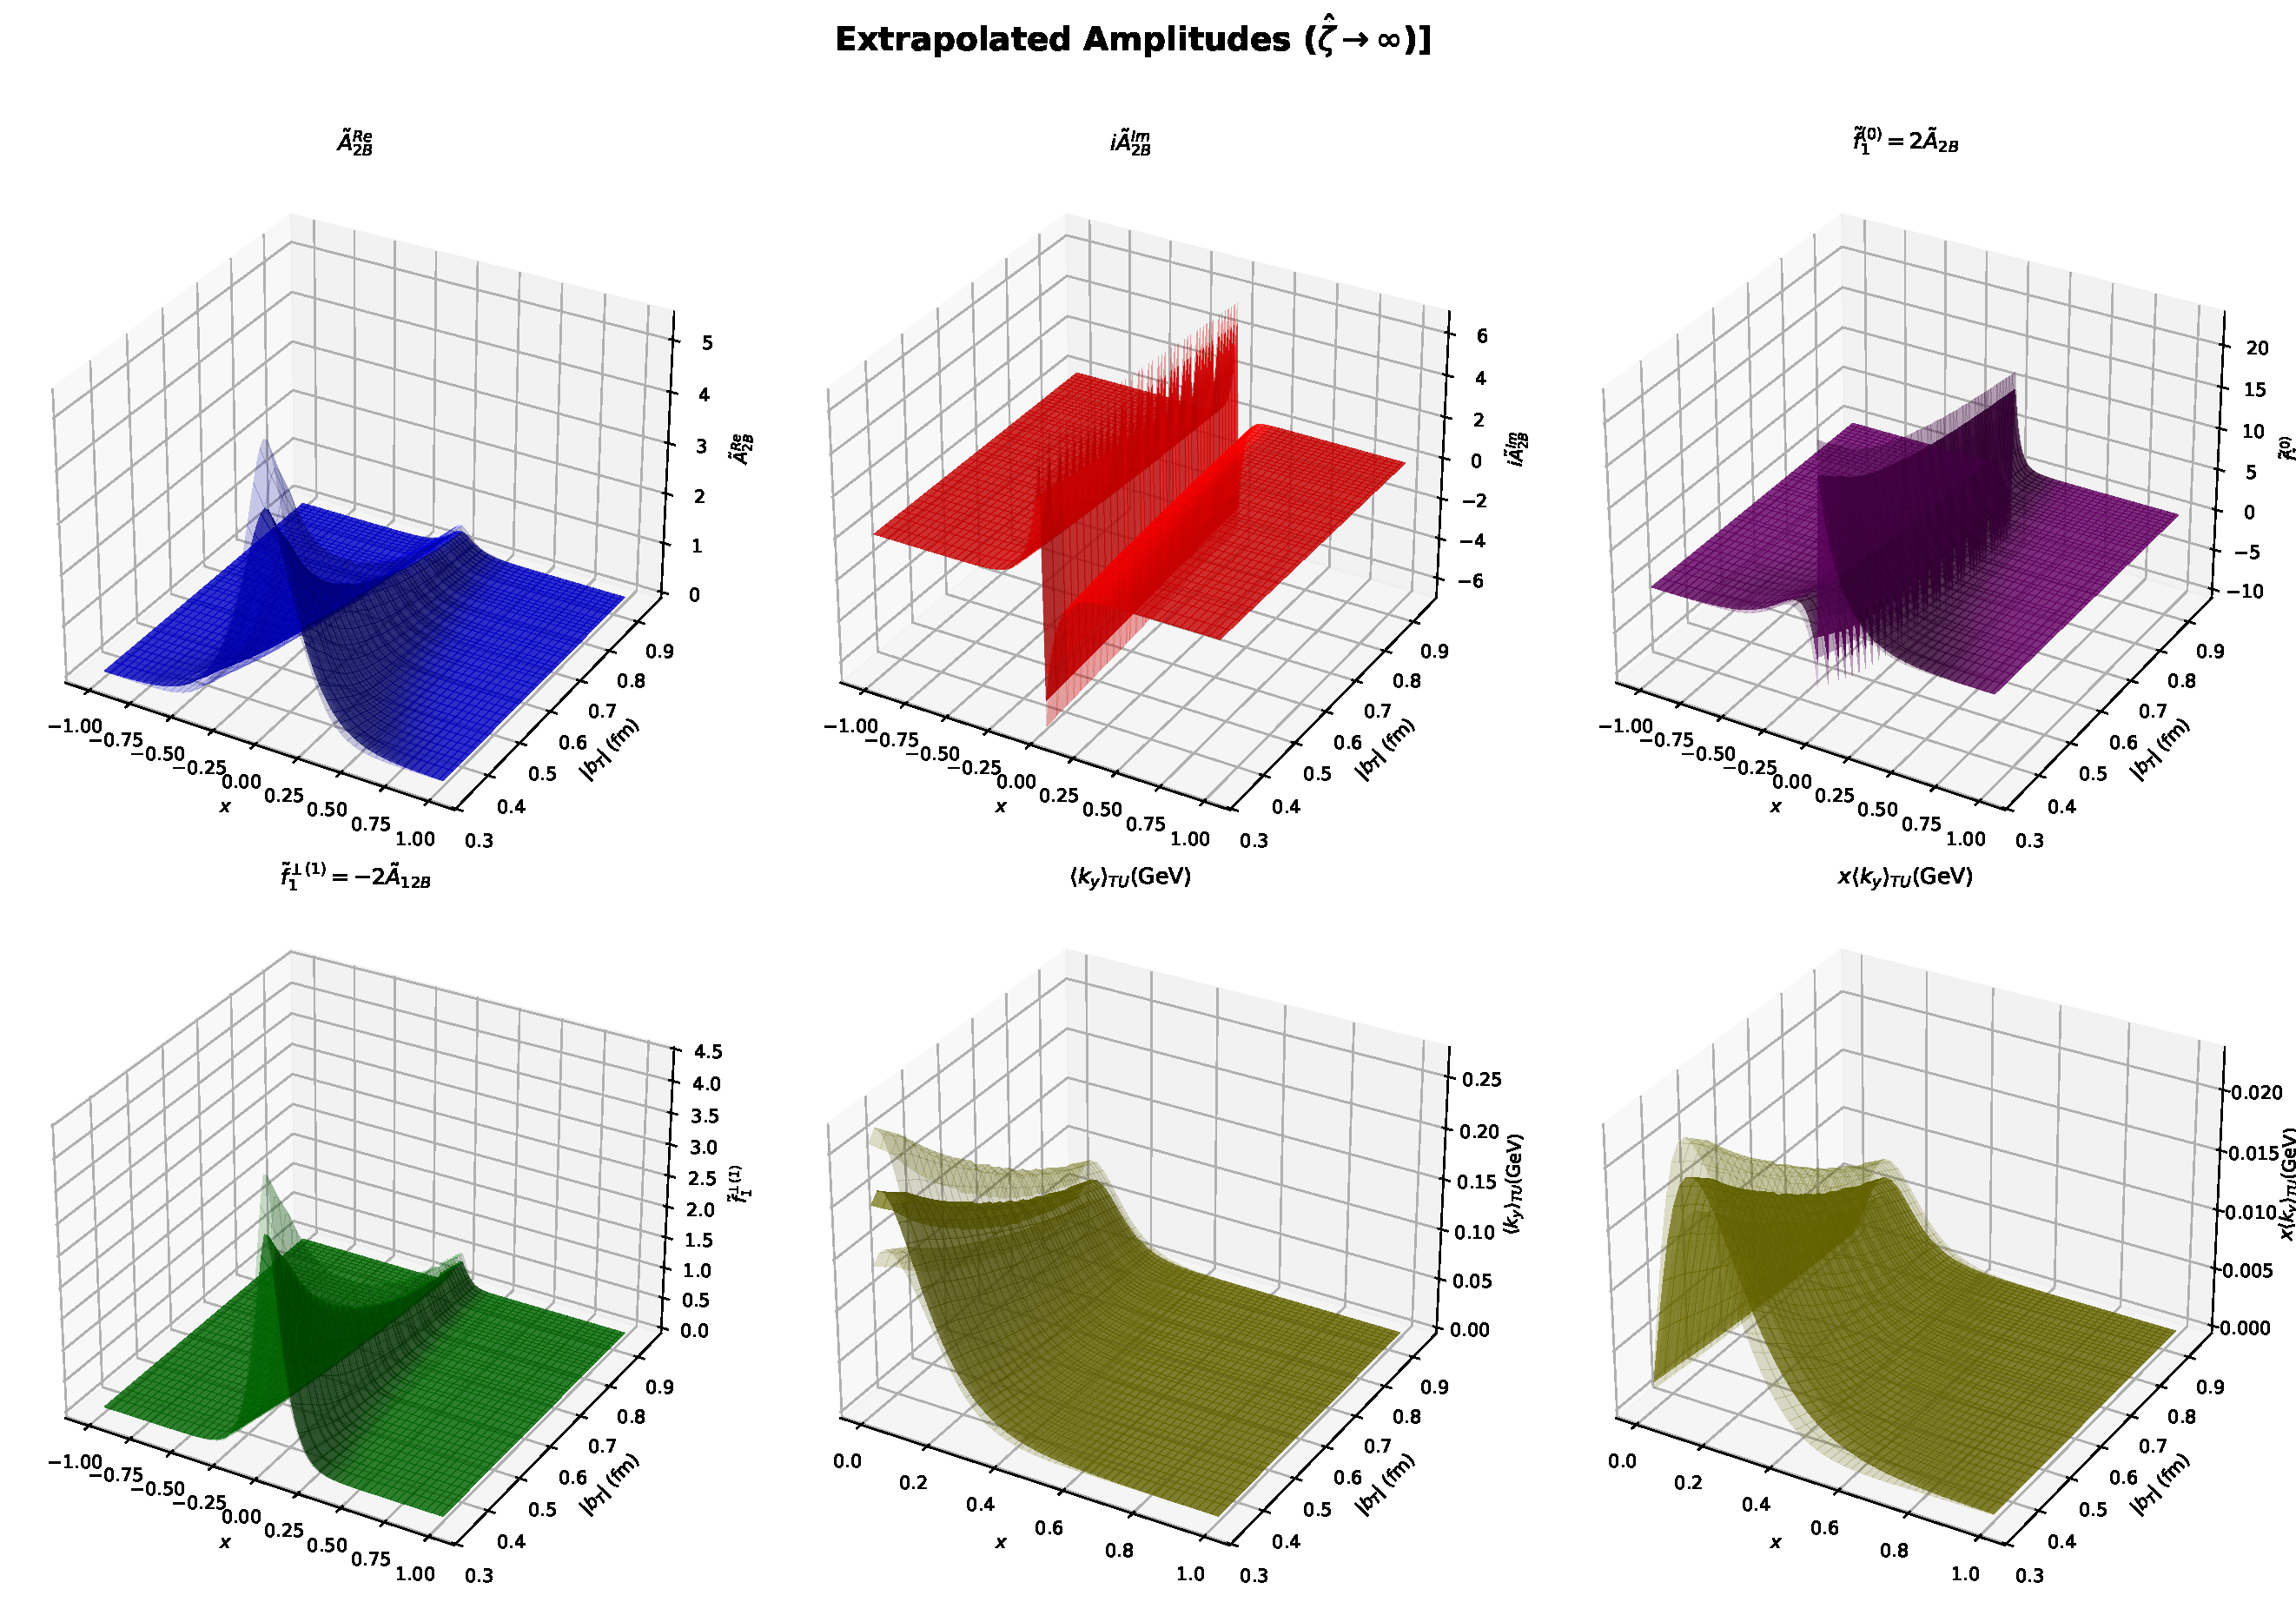
\includegraphics[width=0.8\linewidth]{SimultaneousFitsCov/extrapolation_para_level/SimulFitCovMatrix-A12B-A2B-FT-3D__bmin3_eta610_PLInf.pdf}
    \caption{The same six extrapolated ($\hat\zeta\to\infty$) quantities as Fig.~\ref{fig:extrapolated_amplitude_level}, shown here as full surfaces in $x$ and transverse separation $|b_T|$ (ranging from $3a\approx0.34$ fm to $\sqrt{68}\,a\approx0.94$ fm). The joint $x$-$|b_T|$ dependence illustrates how the reconstructed amplitudes and the extracted Sivers shift evolve with transverse quark separation at the physical limit.}
    \label{fig:extrapolated_amplitude_3d}
\end{figure}

\begin{figure}[h!]
    \centering
    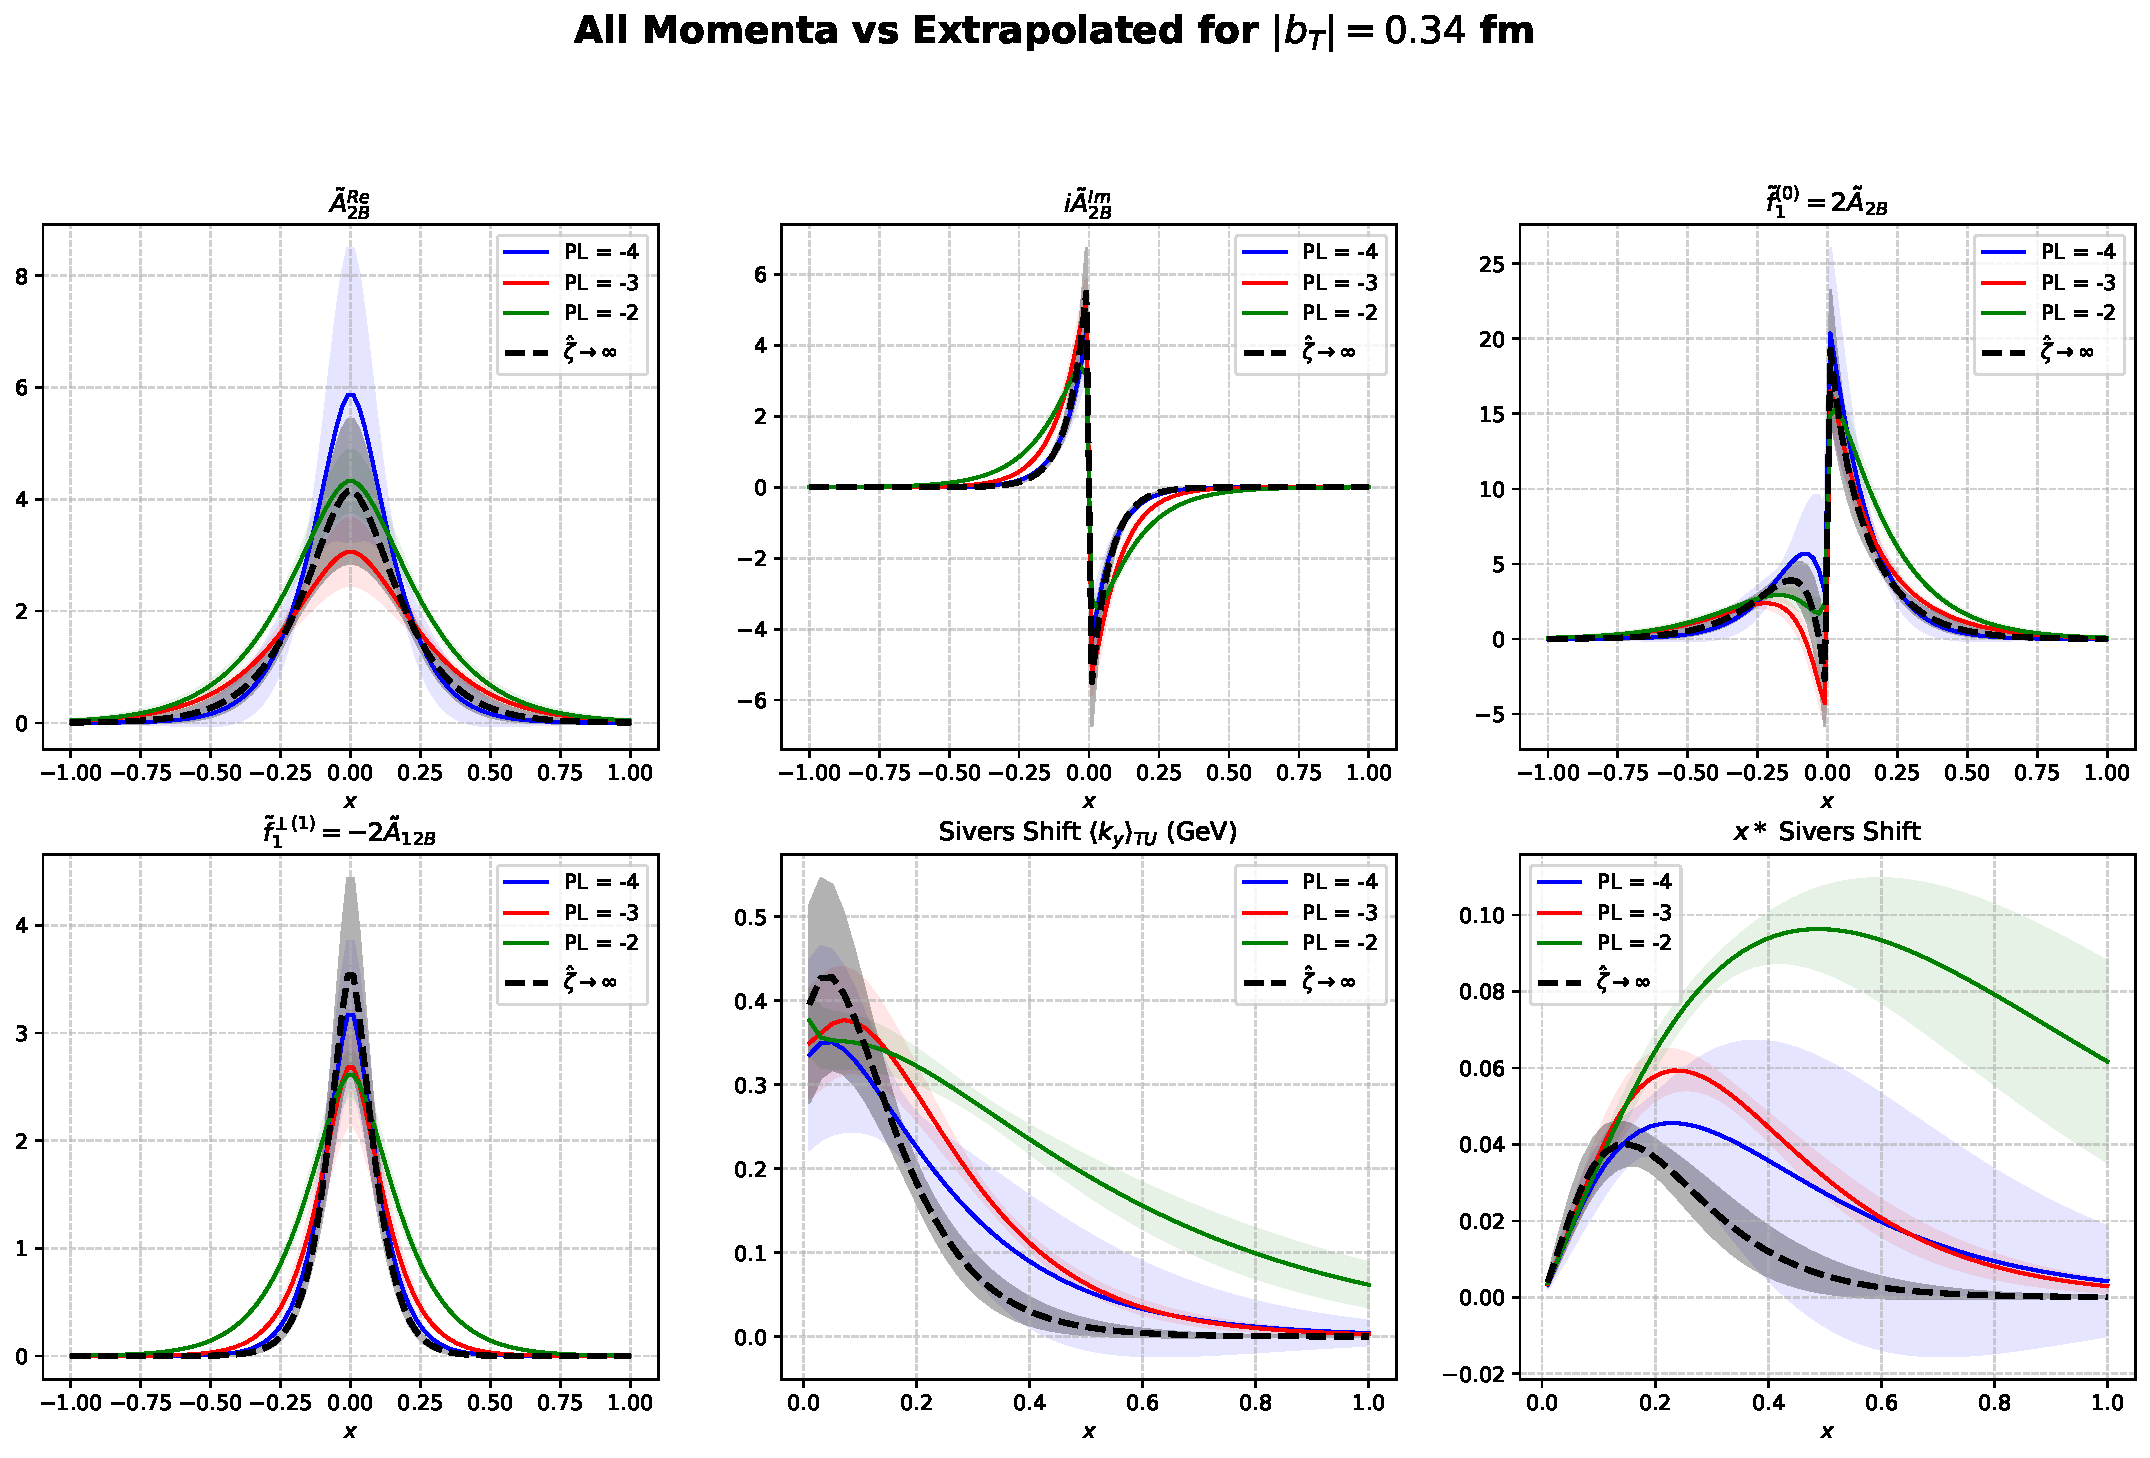
\includegraphics[width=0.8\linewidth]{SimultaneousFitsCov/extrapolation_para_level/All_Momenta_vs_Extrapolated_2D_P234_bmin3_eta610_b29.0.pdf}
    \caption{Comparison, at fixed $|b_T| = 3a \approx 0.34$ fm, between the six physical quantities evaluated at each of the three finite momenta used in the extrapolation ($P_L=-2,-3,-4$, colored curves, each using its own unextrapolated fit parameters) and the extrapolated $\hat\zeta\to\infty$ result (black dashed curve). The extrapolated curve is distinct from all three finite-momentum curves rather than coinciding with the largest simulated momentum, confirming that the fit-parameter extrapolation of Fig.~\ref{fig:param_extrapolation_zetahat} captures genuine momentum dependence rather than simply reproducing the $P_L=-4$ result.}
    \label{fig:momenta_vs_extrapolated}
\end{figure}

\subsection{Testing Factorization in \texorpdfstring{$x$}{TEXT} and \texorpdfstring{$|b_T|$}{TEXT}}
\label{sec:factorization_xbt}

Figures~\ref{fig:extrapolated_amplitude_3d} and~\ref{fig:momenta_vs_extrapolated} show that the extrapolated Sivers shift and amplitudes depend on both $x$ and $|b_T|$ jointly. A natural question is whether this joint dependence is actually separable: does the extrapolated Sivers shift factorize as
\begin{equation}
    \langle k_y \rangle_{TU}(x,|b_T|) \overset{?}{=} F(x)\,G(|b_T|) \ ,
\end{equation}
with all of the $x$-shape carried by $F(x)$ and all of the $|b_T|$-shape by $G(|b_T|)$? Such a factorization is not automatic in our fit ansatz. Each amplitude enters only through the combination $d_X(b^2) = 1 + d_X\,b^2$ inside a Bessel function that also carries the $x$-dependence,
\begin{equation}
    \tAmp_X(x,b^2) \ \propto\ N_X(b^2)\ |x|^{-1/2+j_X}\ K_{\nu_X}\!\left(|x|\sqrt{d_X(b^2)/c_X}\right) \ ,
\end{equation}
so $|b_T|$ rescales the argument of the same Bessel function that carries the $x$-dependence, rather than multiplying it by an overall $x$-independent prefactor. The Sivers shift is a ratio of three such amplitudes ($\tAmp_{2B}^{\text{Re}}$, $\tAmp_{2B}^{\text{Im}}$, $\tAmp_{12B}^{\text{Re}}$), each with its own independently fitted $(j_X,d_X)$; an exact factorization would require these parameters to coincide across the three amplitudes so that the $x$- and $|b_T|$-dependence separates cleanly. Whether the extrapolated fit lands close enough to that coincidence is a numerical question, which we answer quantitatively below.

\subsubsection{Quantifying the Distance from a Factorized Form}
\label{sec:factorization_metric}

Given a function of two variables $f(x,|b_T|)$, we quantify how far it is from a factorized form $g(x)h(|b_T|)$ by finding the closest such pair in the least-squares sense and reporting the residual. Explicitly, we minimize
\begin{equation}
    J = \int dx\, d|b_T| \, \big(f(x,|b_T|) - g(x)h(|b_T|)\big)^2
\end{equation}
over all functions $g$ and $h$. Setting the functional derivatives with respect to $g(x)$ and $h(|b_T|)$ to zero gives
\begin{align}
    0 &= \frac{\delta J}{\delta g(x)} = \int d|b_T|\, f(x,|b_T|)\,h(|b_T|) - g(x)\int d|b_T|\, h^2(|b_T|) \ , \\
    0 &= \frac{\delta J}{\delta h(|b_T|)} = \int dx\, f(x,|b_T|)\,g(x) - h(|b_T|)\int dx\, g^2(x) \ ,
\end{align}
which can be solved for $h$ in terms of $g$,
\begin{equation}
    h(|b_T|) = \frac{\int dx\, f(x,|b_T|)\,g(x)}{\int dx\, g^2(x)} \ ,
    \label{eq:factorization_h_solution}
\end{equation}
and reinserted to eliminate $h$, giving a closed, self-consistent equation for $g$ alone:
\begin{equation}
    g(x) = \left[\int d|b_T| \left[\frac{\int dx'\, f(x',|b_T|)\,g(x')}{\int dx'\, g^2(x')}\right]^2\right]^{-1} \int d|b_T|\, f(x,|b_T|)\,\frac{\int dx'\, f(x',|b_T|)\,g(x')}{\int dx'\, g^2(x')} \ .
    \label{eq:factorization_g_selfconsistent}
\end{equation}
Equation~\eqref{eq:factorization_g_selfconsistent} is solved iteratively: starting from an initial guess $g=1$, the right-hand side is evaluated to obtain a refined $g$, which is reinserted, and the process repeated until $g$ (and the resulting relative distance below) stops changing to within a fixed tolerance. Convergence is rapid in practice, typically within 4-6 iterations for the grids used here.

Having found the optimal separable pair $g(x)h(|b_T|)$, we compare its residual $\sqrt{J}$ to the overall size of $f$ itself, $N = \int dx\, d|b_T|\, f^2(x,|b_T|)$, giving the relative distance from a factorized form:
\begin{equation}
    \text{relative distance} = \sqrt{J/N} \ .
    \label{eq:factorization_relative_distance}
\end{equation}
A relative distance of zero indicates exact factorization; the closer to zero, the better $F(x)G(|b_T|)$ approximates the true joint $(x,|b_T|)$ dependence. In practice, we replace the continuum integrals with sums over a discrete $(x,|b_T|)$ grid, apply the iteration of Eq.~\eqref{eq:factorization_g_selfconsistent} independently to each Jackknife sample of the extrapolated amplitudes, and reduce the resulting distribution of relative distances to a Jackknife mean and error. We repeat the full test in four $x$-windows, $[0,1]$, $[0.1,0.9]$, $[0.2,0.8]$, and $[0.3,0.8]$, to check that the conclusion is not an artifact of the amplitudes' behavior near $x=0$.

\subsubsection{Factorization Test for the Sivers Shift}
\label{sec:factorization_sivers_test}

Before running the distance test itself, we can already see that exact factorization is unlikely from the extrapolated fit parameters directly. As noted in Section~\ref{sec:factorization_xbt}, factorization requires the Bessel-function order $j_X$ and width parameter $d_X$ to coincide across the three input amplitudes; the extrapolated values are
\begin{equation}
    j_{\text{re}} = 2.0667(69), \quad j_{\text{im}} = 0.9921(92), \quad j_{\text{reA12B}} = 2.0026(40) \ ,
\end{equation}
\begin{equation}
    d_{\text{re}} = 0.139(12), \quad d_{\text{im}} = 0.183(14), \quad d_{\text{reA12B}} = 0.105(18) \ .
\end{equation}
The two $j$ parameters entering the real amplitudes, $j_{\text{re}}$ and $j_{\text{reA12B}}$, agree with each other, but $j_{\text{im}} \approx 1$ is clearly distinct from both; the three $d$ parameters are closer to each other but still resolved from one another well outside their Jackknife uncertainties. This parameter-level mismatch, particularly in $j$, is a concrete, independent reason to expect a nonzero residual from exact factorization.

Table~\ref{tab:factorization_sivers} lists the resulting relative distance of the extrapolated Sivers shift $\langle k_y \rangle_{TU}(x,|b_T|)$ from its best separable approximation, over $|b_T| \in [0.3421,0.9403]$ fm (60 points, fixed across all four $x$-windows).

\begin{table}[h!]
    \centering
    \renewcommand{\arraystretch}{1.4}
    \caption{Relative distance of the extrapolated Sivers shift $\langle k_y \rangle_{TU}(x,|b_T|)$ from its optimal factorized approximation $F(x)G(|b_T|)$, Eq.~\eqref{eq:factorization_relative_distance}, over $|b_T| \in [0.3421, 0.9403]$ fm for four choices of $x$-window.}
    \label{tab:factorization_sivers}
    \begin{tabular}{|c|c|c|}
    \hline
    $x$-window & ALS iterations to converge & Relative distance \\
    \hline
    $[0.0,1.0]$ & 4 & $0.0568(78)$ \\
    \hline
    $[0.1,0.9]$ & 5 & $0.0714(95)$ \\
    \hline
    $[0.2,0.8]$ & 5 & $0.0758(75)$ \\
    \hline
    $[0.3,0.8]$ & 4 & $0.0620(88)$ \\
    \hline
    \end{tabular}
\end{table}

In every window the relative distance is nonzero well outside its Jackknife uncertainty, at the level of $6$-$8\%$: the Sivers shift is close to, but not exactly, factorized, and this residual is stable under narrowing the $x$-window away from $x=0$ rather than being driven by behavior at the endpoint. Figure~\ref{fig:factorization_gh_sivers} shows the resulting optimal separable factors $g(x)$ and $h(|b_T|)$ for all four windows together with the quality of the $g(x)h(|b_T|)$ reconstruction against the actual data at the two extreme $|b_T|$ values in the fit range.

\begin{figure}[h!]
    \centering
    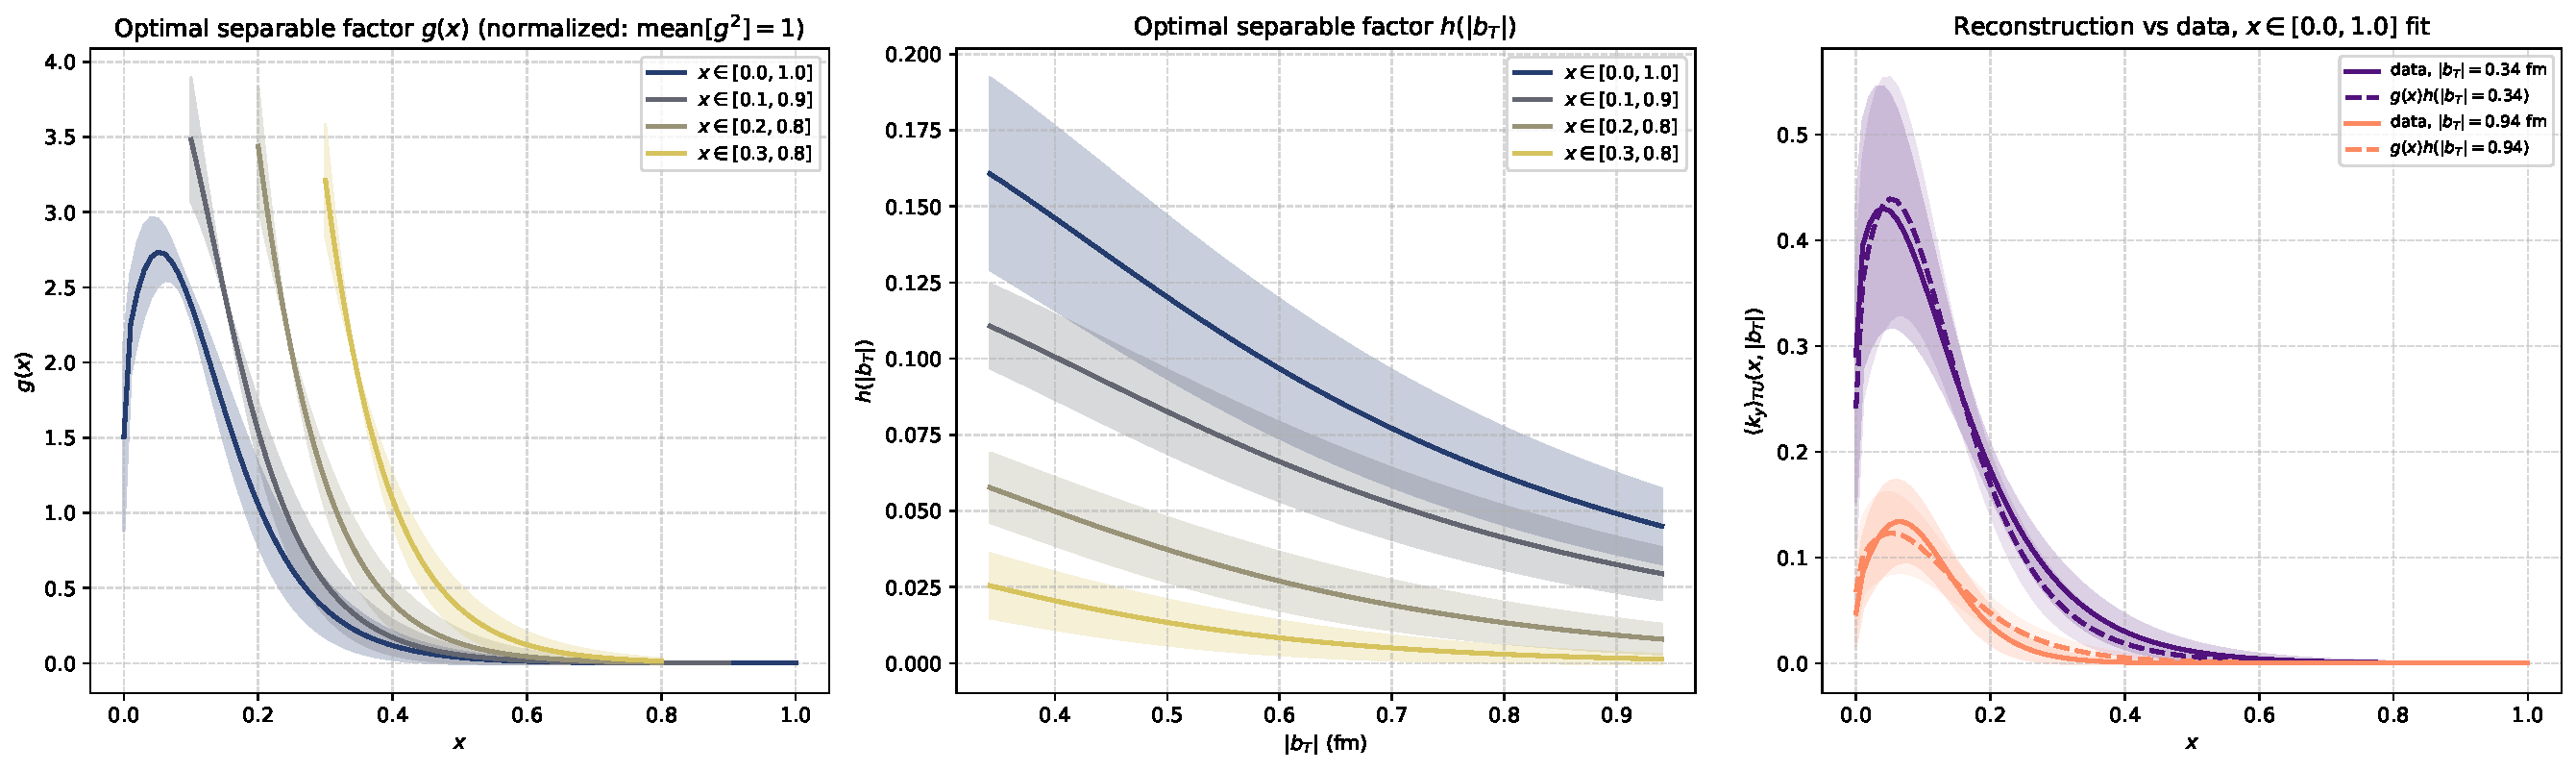
\includegraphics[width=\linewidth]{SimultaneousFitsCov/factorization_test/Factorization_gh_and_Reconstruction_bmin3_eta610.pdf}
    \caption{Left and center: the optimal separable factors $g(x)$ and $h(|b_T|)$ (Eqs.~\eqref{eq:factorization_h_solution}-\eqref{eq:factorization_g_selfconsistent}, normalized so $\text{mean}[g^2]=1$) for the extrapolated Sivers shift, shown for all four $x$-windows of Table~\ref{tab:factorization_sivers}. Right: the reconstructed $g(x)h(|b_T|)$ (dashed) compared to the actual extrapolated Sivers shift (solid) at the smallest and largest fitted $|b_T|$, using the $x\in[0,1]$ fit; the visible gap between the solid and dashed curves is the residual quantified in Table~\ref{tab:factorization_sivers}.}
    \label{fig:factorization_gh_sivers}
\end{figure}

A complementary, more direct way to see the same non-factorization is to form explicit ratios of the Sivers shift at fixed $x$ or fixed $|b_T|$. If $\langle k_y \rangle_{TU}(x,|b_T|) = F(x)G(|b_T|)$ exactly, then $R_b(x) \equiv \langle k_y \rangle_{TU}(x,|b_T|)/\langle k_y \rangle_{TU}(x,|b_T|_{\text{ref}}) = G(|b_T|)/G(|b_T|_{\text{ref}})$ must be flat in $x$ for every choice of $|b_T|$ and reference $|b_T|_{\text{ref}}$, and likewise $R_x(|b_T|) \equiv \langle k_y \rangle_{TU}(x,|b_T|)/\langle k_y \rangle_{TU}(x_{\text{ref}},|b_T|) = F(x)/F(x_{\text{ref}})$ must be flat in $|b_T|$ for every $x$ and $x_{\text{ref}}$; requiring this for every pair of references is not just necessary but sufficient for factorization, so it is a complete test rather than a heuristic proxy. Figures~\ref{fig:factorization_ratio_x_sivers} and~\ref{fig:factorization_ratio_bT_sivers} show that neither ratio is flat.

\begin{figure}[h!]
    \centering
    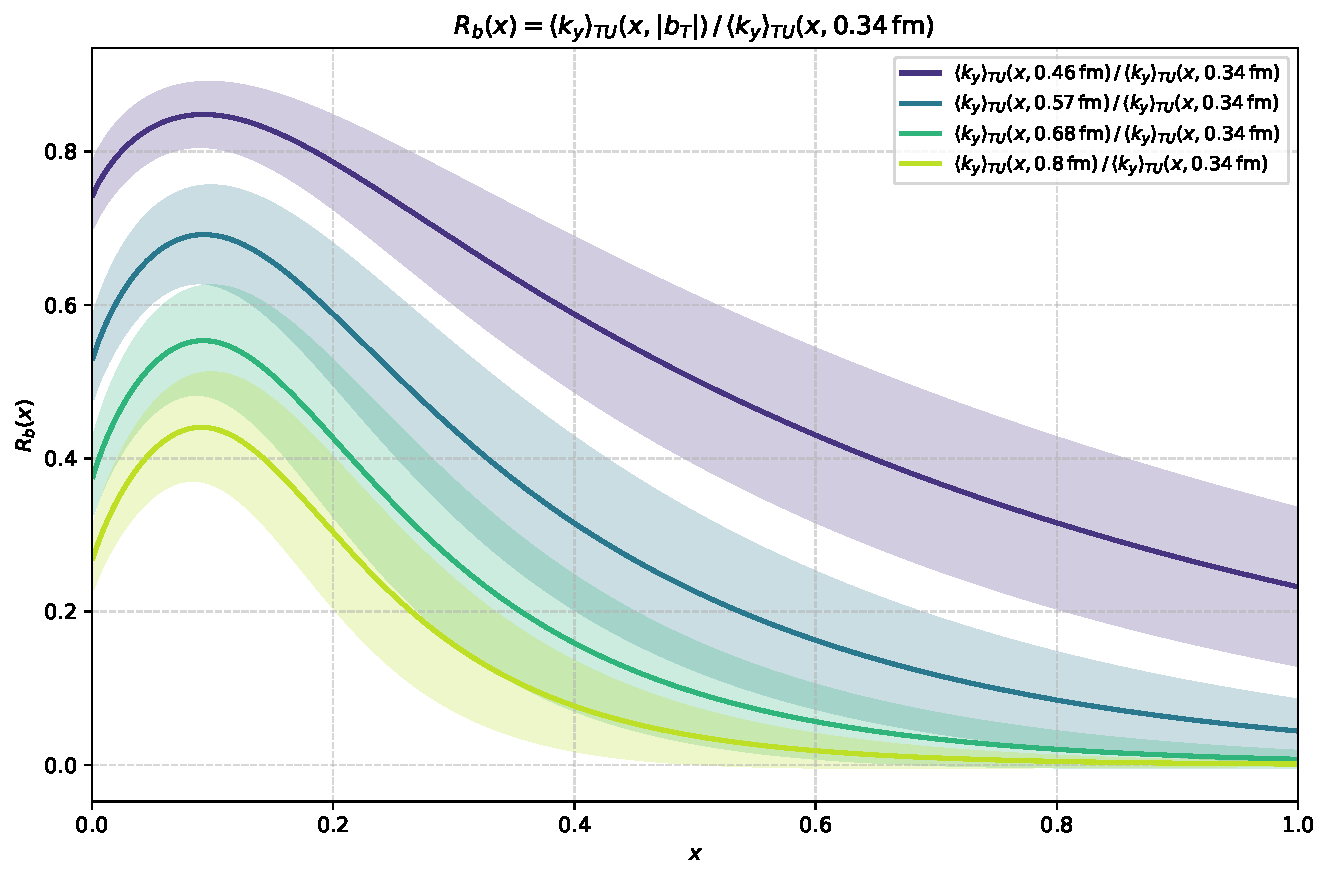
\includegraphics[width=0.75\linewidth]{SimultaneousFitsCov/factorization_test/Factorization_Ratio_vs_x_4curves_P234_bmin3_eta610.pdf}
    \caption{$R_b(x) = \langle k_y \rangle_{TU}(x,|b_T|)/\langle k_y \rangle_{TU}(x,0.34\text{ fm})$ for four values of $|b_T|$, as a function of $x$. Under exact factorization each curve would be flat; instead every curve rises from its $x\to0$ value to a peak near $x\approx0.1$ before decaying, showing that the $|b_T|$-dependence of the Sivers shift is itself $x$-dependent.}
    \label{fig:factorization_ratio_x_sivers}
\end{figure}

\begin{figure}[h!]
    \centering
    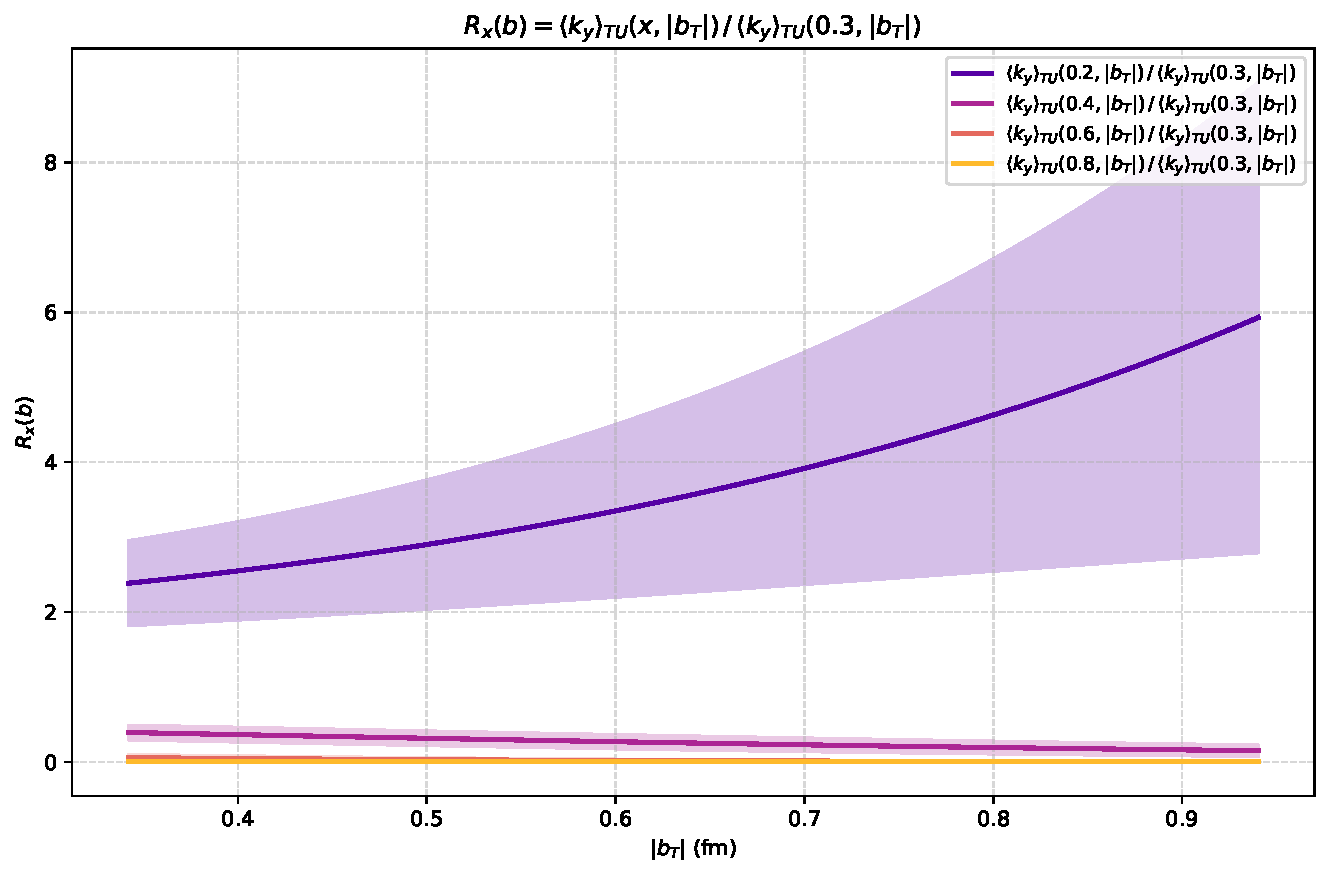
\includegraphics[width=0.75\linewidth]{SimultaneousFitsCov/factorization_test/Factorization_Ratio_vs_bT_4curves_P234_bmin3_eta610.pdf}
    \caption{$R_x(|b_T|) = \langle k_y \rangle_{TU}(x,|b_T|)/\langle k_y \rangle_{TU}(0.3,|b_T|)$ for four values of $x$, as a function of $|b_T|$. The $x=0.2$ curve varies by more than a factor of two across the fitted $|b_T|$ range rather than remaining flat, confirming that the $x$-dependence of the Sivers shift is itself $|b_T|$-dependent, consistent with Fig.~\ref{fig:factorization_ratio_x_sivers}.}
    \label{fig:factorization_ratio_bT_sivers}
\end{figure}

Finally, we check that this non-factorization is not an artifact introduced by the $\hat\zeta\to\infty$ extrapolation itself, by repeating the $R_b(x)$ and $R_x(|b_T|)$ ratio tests directly on the raw, unextrapolated fit parameters at each individual finite momentum. Figures~\ref{fig:factorization_ratio_x_finitePL} and~\ref{fig:factorization_ratio_bT_finitePL} show that the same qualitative pattern, non-flat ratios in both $x$ and $|b_T|$, is already present at every simulated momentum, and if anything becomes more pronounced at the higher momenta.

\begin{figure}[h!]
    \centering
    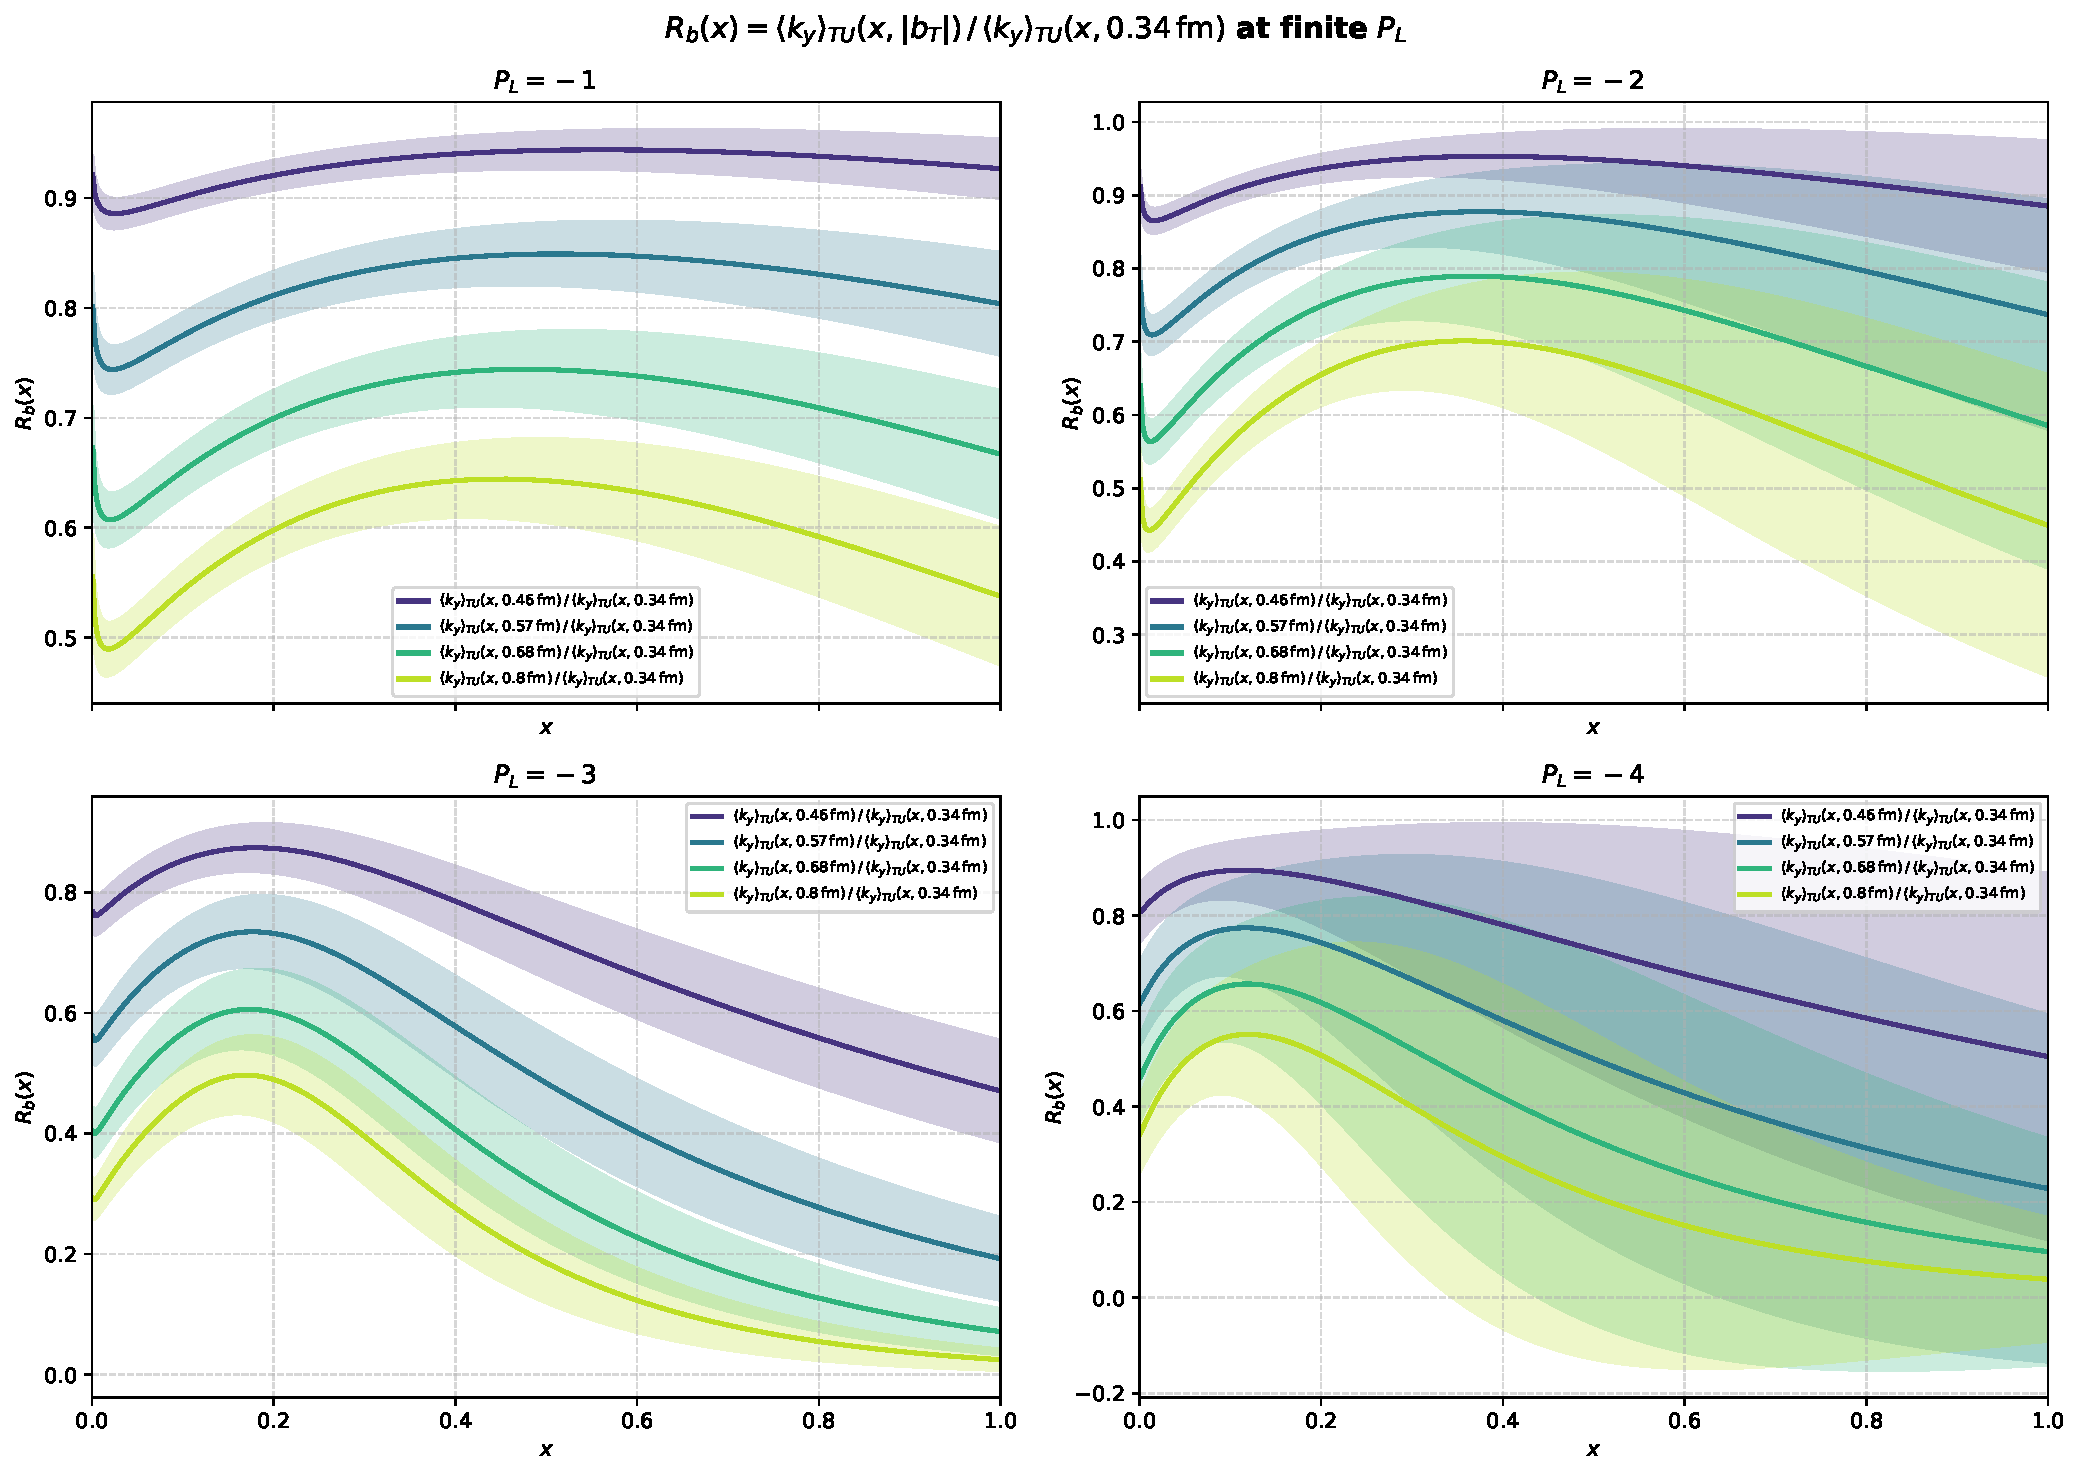
\includegraphics[width=\linewidth]{SimultaneousFitsCov/factorization_test/Factorization_Ratio_vs_x_AllPL_bmin3_eta610.pdf}
    \caption{The same ratio test as Fig.~\ref{fig:factorization_ratio_x_sivers}, $R_b(x)$, repeated at each finite momentum individually using its own raw (unextrapolated) fit parameters. None of the four panels shows a flat curve, confirming that the non-factorization is a genuine feature of the fitted amplitudes rather than an artifact of the $\hat\zeta\to\infty$ extrapolation.}
    \label{fig:factorization_ratio_x_finitePL}
\end{figure}

\begin{figure}[h!]
    \centering
    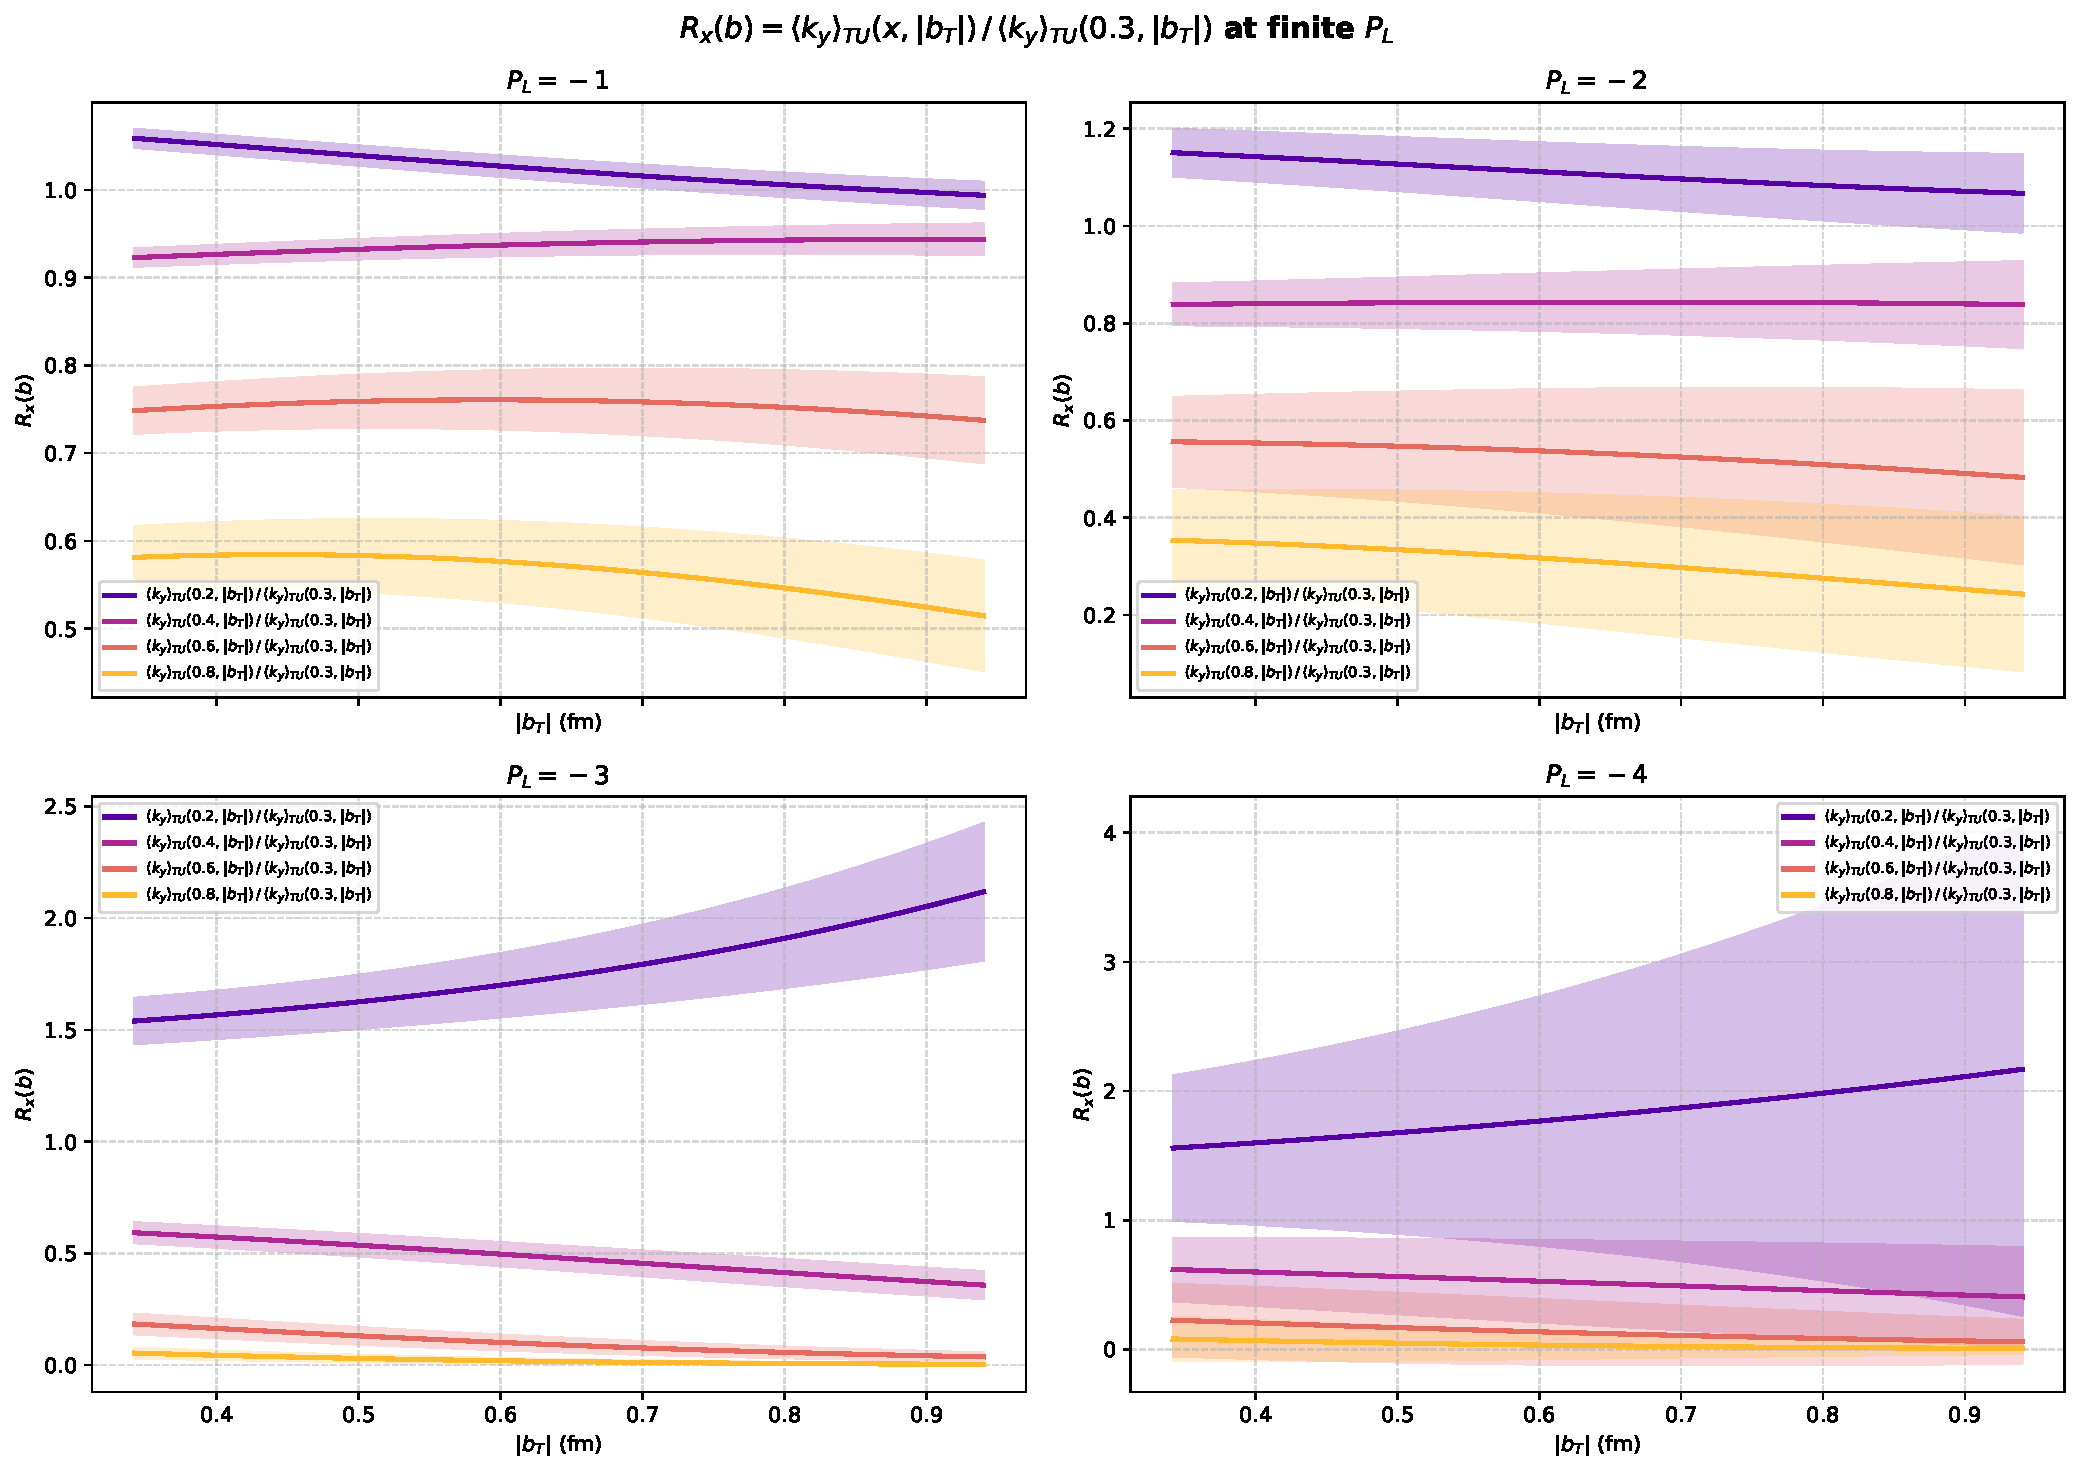
\includegraphics[width=\linewidth]{SimultaneousFitsCov/factorization_test/Factorization_Ratio_vs_bT_AllPL_bmin3_eta610.pdf}
    \caption{The same ratio test as Fig.~\ref{fig:factorization_ratio_bT_sivers}, $R_x(|b_T|)$, repeated at each finite momentum individually. The departure from flatness grows with $|P_L|$, most visibly in the $x=0.2$ curve, which is consistent with the parameter mismatch identified in the extrapolated $j_X$ and $d_X$ values above.}
    \label{fig:factorization_ratio_bT_finitePL}
\end{figure}

\subsubsection{Factorization Test at the Amplitude Level}
\label{sec:factorization_amplitude_test}

The Sivers-shift test above probes factorization of the full ratio $\langle k_y \rangle_{TU} = -m_N \tAmp_{12B}^{\text{Re}}/(\tAmp_{2B}^{\text{Re}} - i\tAmp_{2B}^{\text{Im}})$, in which some of the non-factorized behavior of the individual amplitudes could in principle cancel. We therefore repeat the identical distance test of Section~\ref{sec:factorization_metric} on each extrapolated amplitude separately: $\tAmp_{12B}^{\text{Re}}$, $\tAmp_{2B}^{\text{Re}}$, $i\tAmp_{2B}^{\text{Im}}$, and the combination $\tAmp_{2B}^{\text{Re}} - i\tAmp_{2B}^{\text{Im}}$ (proportional to $\tilde f_1^{[1](0)}$) that appears in the Sivers-shift denominator. Table~\ref{tab:factorization_amplitudes} lists the resulting relative distances, using the same $|b_T|\in[0.3421,0.9403]$ fm grid and four $x$-windows as the Sivers-shift test.

\begin{table}[h!]
    \centering
    \renewcommand{\arraystretch}{1.4}
    \caption{Relative distance of each extrapolated amplitude (and their combination $\tAmp_{2B}^{\text{Re}}-i\tAmp_{2B}^{\text{Im}}$) from its optimal factorized approximation, over the same $|b_T|\in[0.3421,0.9403]$ fm grid and $x$-windows as Table~\ref{tab:factorization_sivers}.}
    \label{tab:factorization_amplitudes}
    \begin{tabular}{|l|c|c|c|c|}
    \hline
    Amplitude & $x\in[0.0,1.0]$ & $x\in[0.1,0.9]$ & $x\in[0.2,0.8]$ & $x\in[0.3,0.8]$ \\
    \hline
    $\tAmp_{12B}^{\text{Re}}$ & $0.0804(18)$ & $0.0573(26)$ & $0.0397(24)$ & $0.0303(21)$ \\
    \hline
    $\tAmp_{2B}^{\text{Re}}$ & $0.08138(65)$ & $0.0718(36)$ & $0.0581(55)$ & $0.0478(56)$ \\
    \hline
    $i\tAmp_{2B}^{\text{Im}}$ & $0.107(18)$ & $0.0868(30)$ & $0.0578(28)$ & $0.0425(23)$ \\
    \hline
    $\tAmp_{2B}^{\text{Re}} - i\tAmp_{2B}^{\text{Im}}$ & $0.1943(63)$ & $0.0926(59)$ & $0.0594(40)$ & $0.0470(47)$ \\
    \hline
    \end{tabular}
\end{table}

Every individual amplitude shows a nonzero relative distance from factorized form in every window, and for the widest window, $x\in[0,1]$, the amplitude-level residuals ($8$-$19\%$) are larger than the corresponding Sivers-ratio residual ($5.7\%$ from Table~\ref{tab:factorization_sivers}): the ratio structure of the Sivers shift partially, but not completely, cancels the non-factorized behavior present in the individual amplitudes. All four amplitude-level residuals shrink as the $x$-window is narrowed away from $x=0$, consistent with each amplitude's own Bessel-function singularity structure near the origin, which differs amplitude by amplitude because of the parameter mismatch identified in Section~\ref{sec:factorization_sivers_test}.

\begin{figure}[h!]
    \centering
    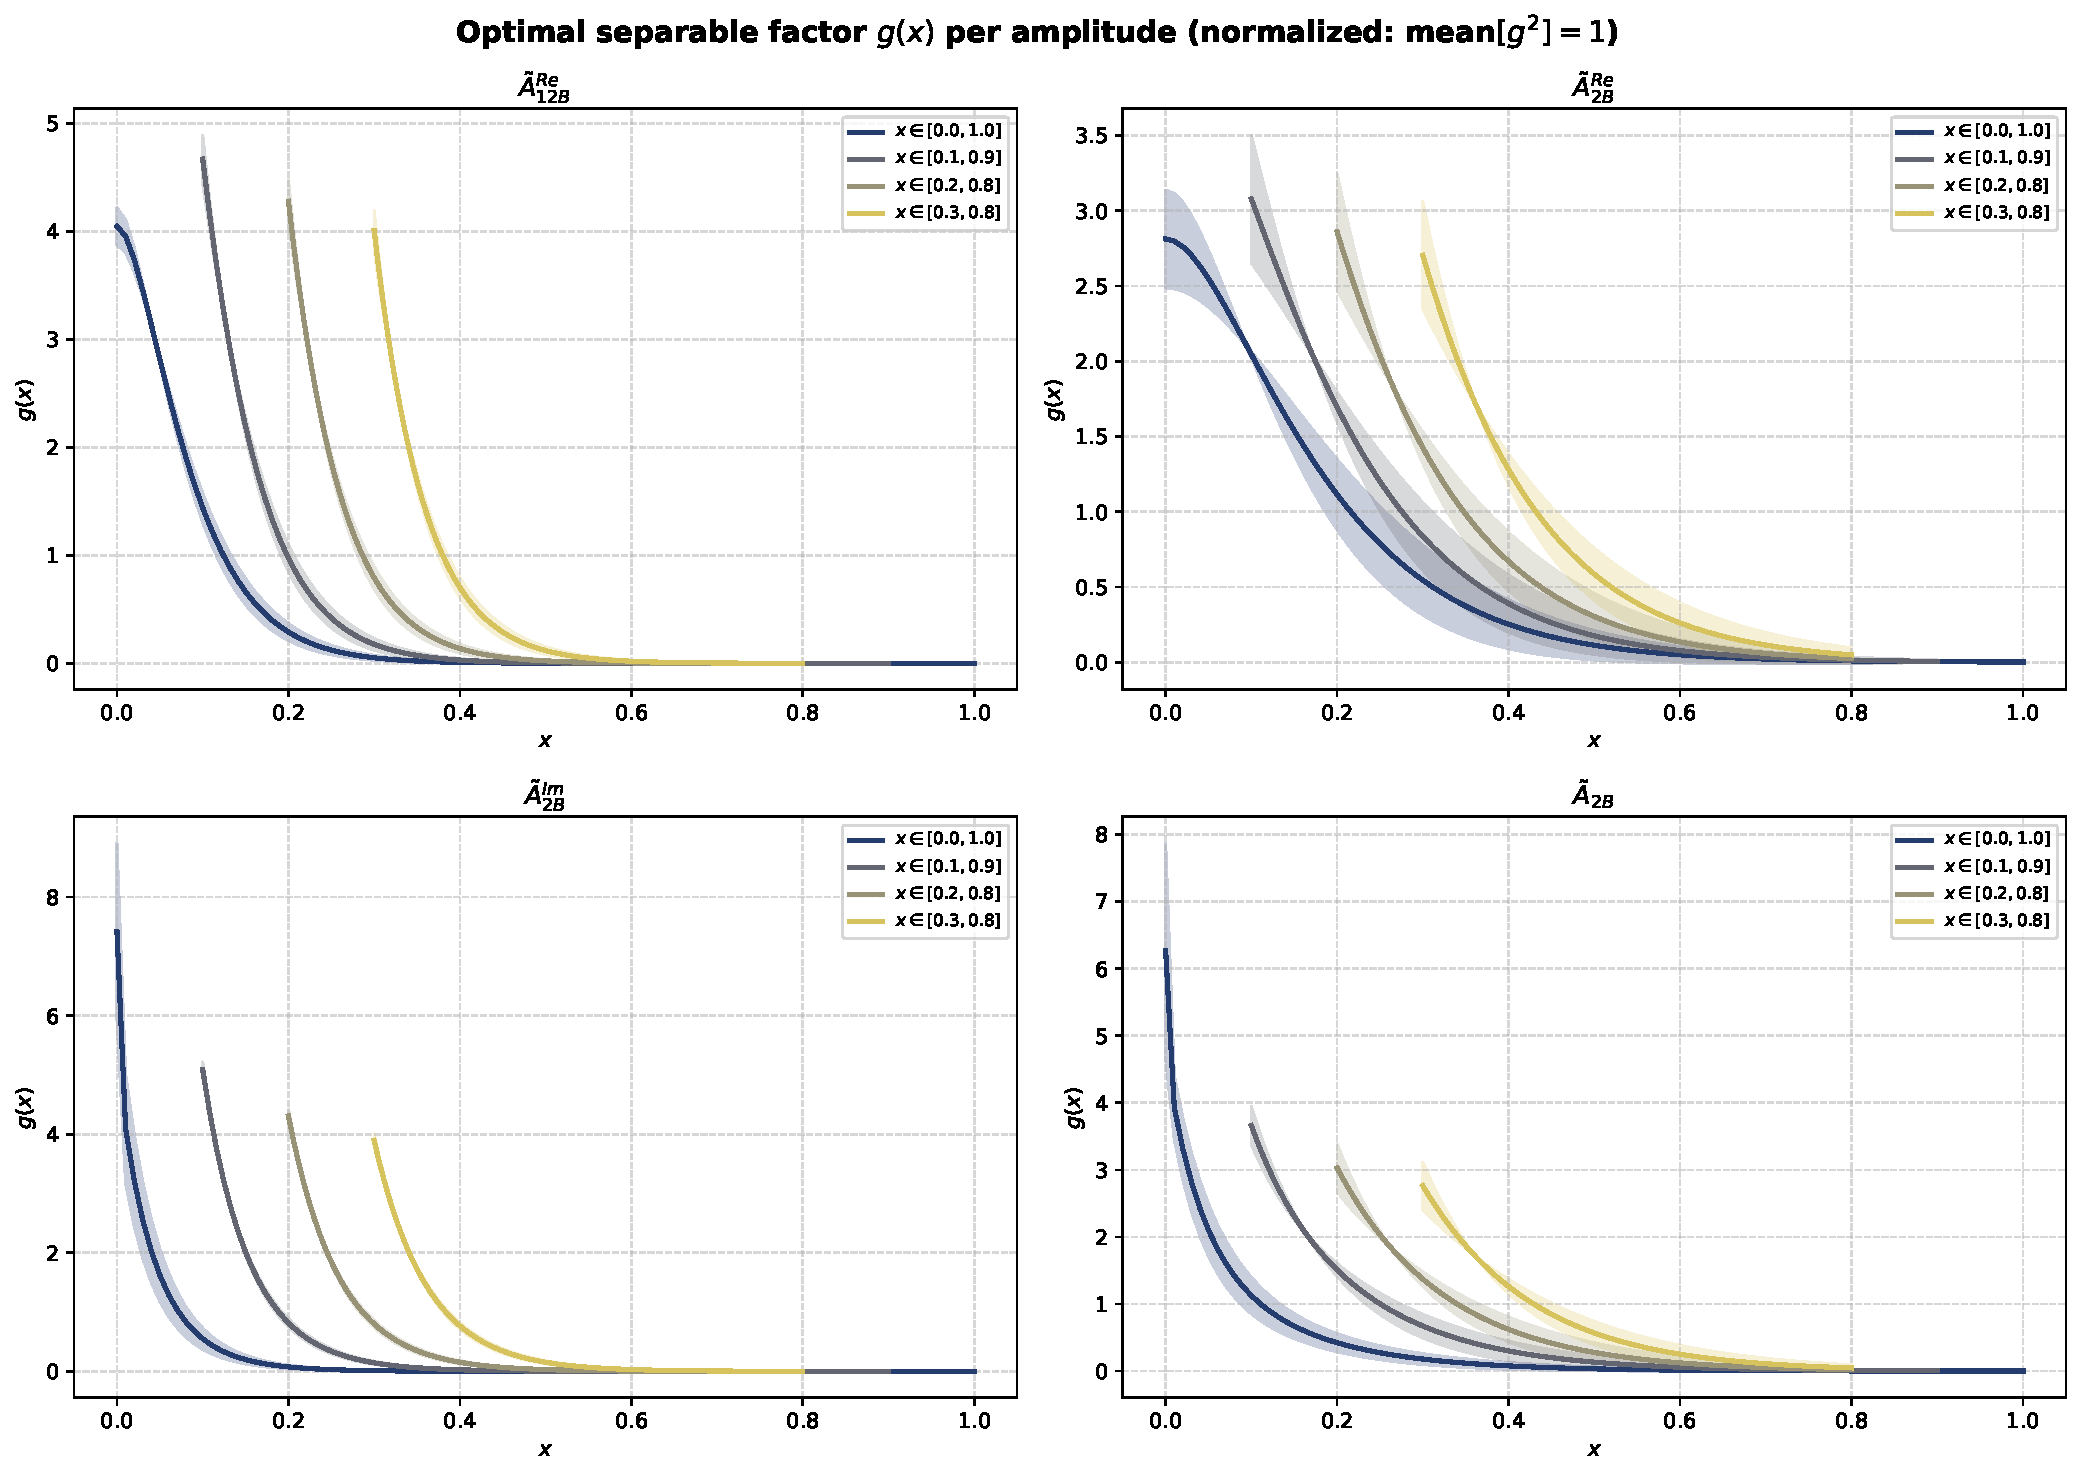
\includegraphics[width=\linewidth]{SimultaneousFitsCov/factorization_test/Factorization_Amplitudes_g_of_x_bmin3_eta610.pdf}
    \caption{Optimal separable factor $g(x)$ for each of the four amplitude combinations of Table~\ref{tab:factorization_amplitudes}, for all four $x$-windows (normalized so $\text{mean}[g^2]=1$). Each amplitude's $g(x)$ is dominated by a sharp rise as $x\to0$ that steepens as the window narrows, reflecting the Bessel-function behavior at small $x$.}
    \label{fig:factorization_g_amplitudes}
\end{figure}

\begin{figure}[h!]
    \centering
    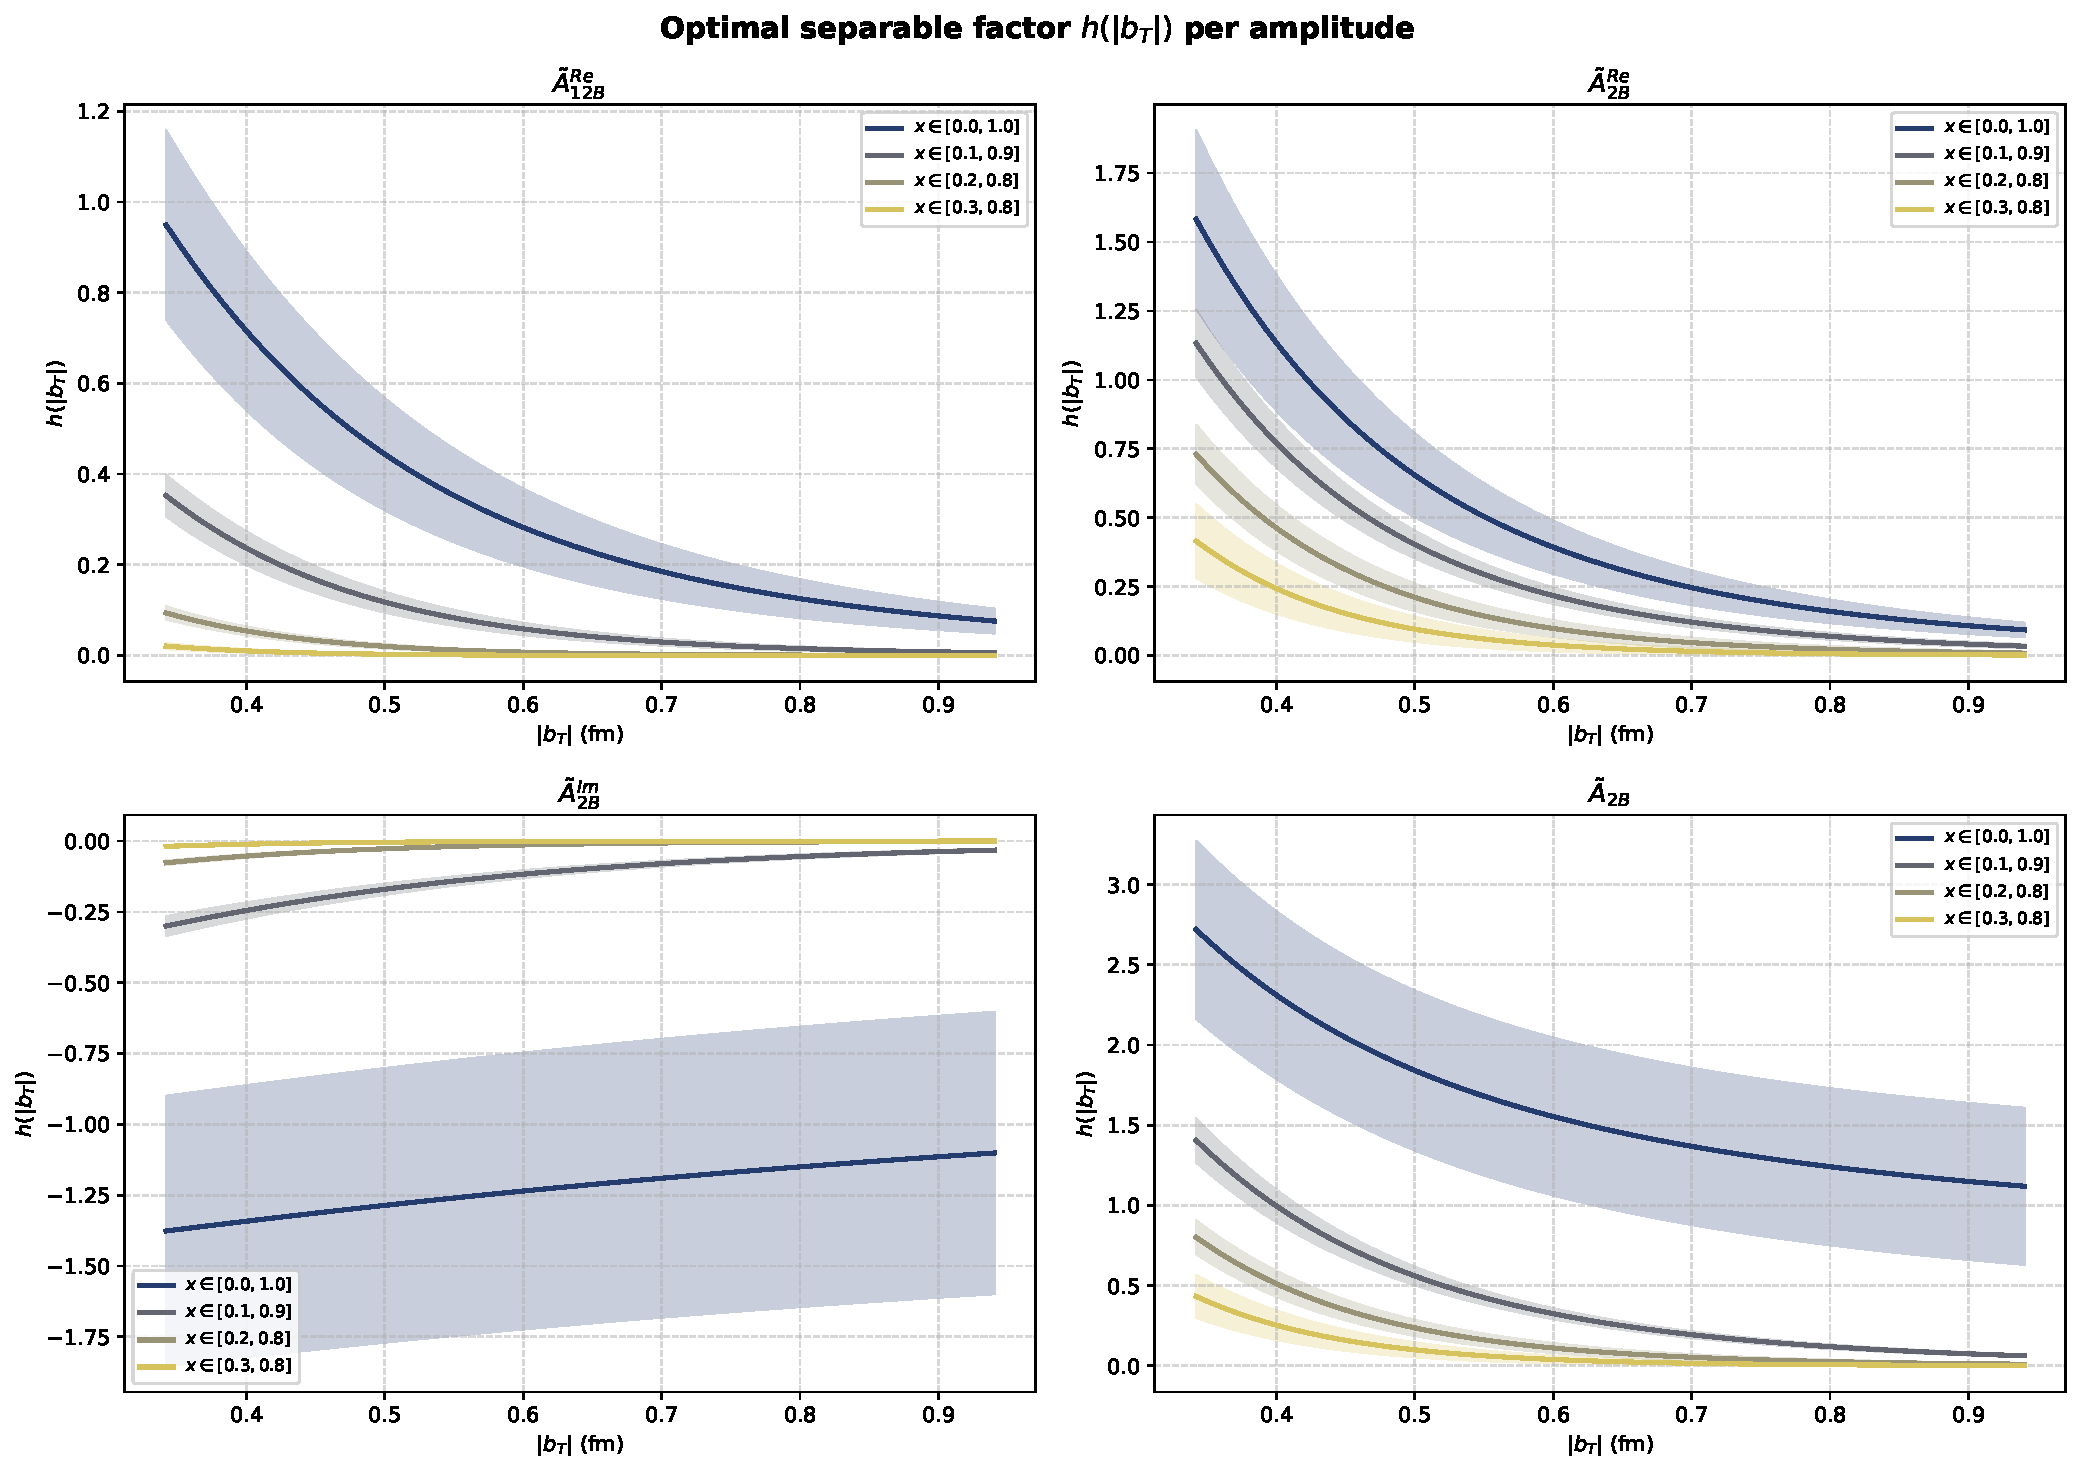
\includegraphics[width=\linewidth]{SimultaneousFitsCov/factorization_test/Factorization_Amplitudes_h_of_bT_bmin3_eta610.pdf}
    \caption{Optimal separable factor $h(|b_T|)$ for each of the four amplitude combinations of Table~\ref{tab:factorization_amplitudes}, for all four $x$-windows. All four amplitudes' $h(|b_T|)$ fall smoothly with increasing $|b_T|$, but with a magnitude and slope that depends on the $x$-window used to define the fit, itself a signature of imperfect factorization.}
    \label{fig:factorization_h_amplitudes}
\end{figure}

\begin{figure}[h!]
    \centering
    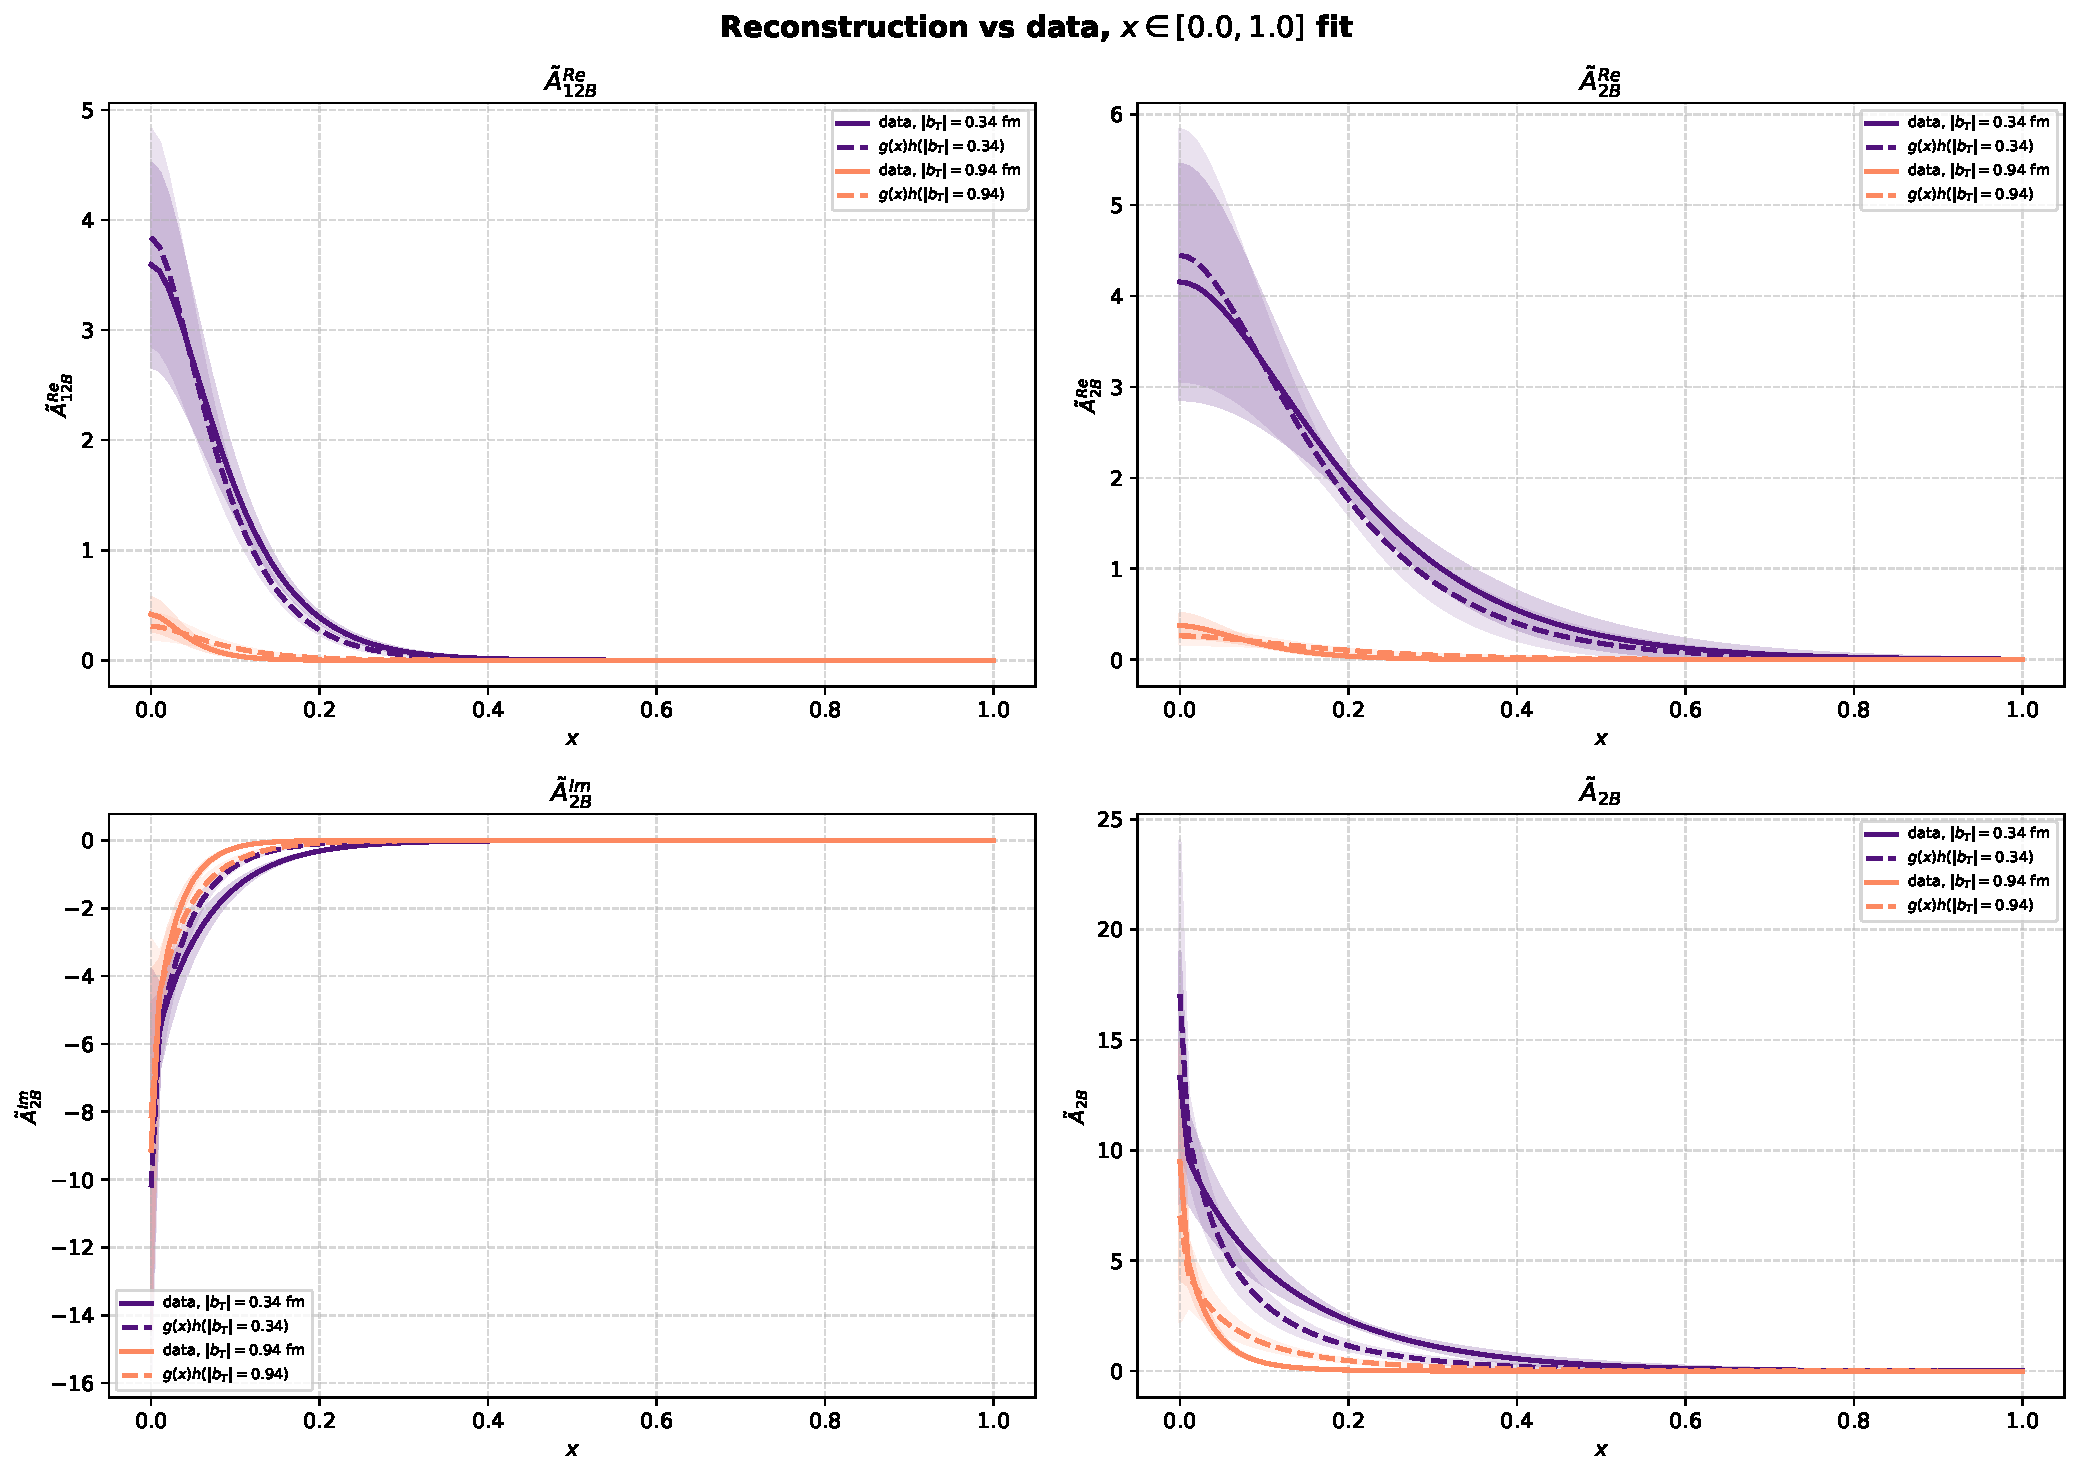
\includegraphics[width=\linewidth]{SimultaneousFitsCov/factorization_test/Factorization_Amplitudes_Reconstruction_bmin3_eta610.pdf}
    \caption{Reconstructed $g(x)h(|b_T|)$ (dashed) against the actual extrapolated amplitude data (solid) at the smallest and largest fitted $|b_T|$, using the $x\in[0,1]$ fit, for each of the four amplitude combinations of Table~\ref{tab:factorization_amplitudes}. The largest reconstruction gap appears near $x\to0$ for every amplitude, matching the $x\in[0,1]$ column of Table~\ref{tab:factorization_amplitudes} being the largest relative distance in every row.}
    \label{fig:factorization_reconstruction_amplitudes}
\end{figure}

Taken together, the Sivers-shift and amplitude-level tests give a consistent picture: neither the individual amplitudes nor the Sivers-shift ratio built from them are exactly factorized in $x$ and $|b_T|$, but the deviation from a factorized form is a modest, well-resolved residual rather than a qualitative failure. The Sivers shift itself is factorized to within roughly $6$-$8\%$ in the relative $L_2$ sense, smaller than the $8$-$19\%$ residuals of the amplitudes that enter it, indicating a partial cancellation of non-factorized behavior in the ratio. This residual is traced directly to the extrapolated fit parameters: the Bessel-function order $j_{\text{im}}\approx1$ governing $\tAmp_{2B}^{\text{Im}}$ differs from $j_{\text{re}},j_{\text{reA12B}}\approx2$ governing the two real amplitudes, and the three width parameters $d_X$ are likewise resolved from one another well outside their Jackknife uncertainties. We conclude that an exactly factorized ansatz $F(x)G(|b_T|)$ would be a good, but not exact, approximation to the extracted Sivers shift.
